%\documentclass[11pt]{scrartcl}
%\documentclass[11pt, twoside, a4paper, BCOR8mm, DIV12, bibtotoc,idxtotoc]{scrbook}
\documentclass[11pt, twoside, a4paper, BCOR8mm, DIV12, bibtotoc,idxtotoc]{scrbook}
\usepackage{german}
\usepackage{typearea}
\usepackage[utf8]{inputenc}
\usepackage{longtable}
\usepackage{hyperref}
\usepackage{graphicx}

% Zusaetzliche Picture-Umgebungen (z.B. shadowenv)
\usepackage{picins}

% Header anpassbar
\usepackage{fancyhdr}

% Headings umdefinieren
\pagestyle{fancy}
\fancyhf{}
\fancyhead[RO]{\nouppercase{\rightmark}}
\fancyhead[LE]{\nouppercase{\leftmark}}
\fancyfoot[RO, LE]{\thepage}

\parindent0.0mm
\parskip0.3cm    
\typearea{13}

\addtolength{\headheight}{7mm}
\addtolength{\headwidth}{1cm}

\addtolength{\oddsidemargin}{11mm}
\addtolength{\evensidemargin}{-11mm}

\begin{document}

\frontmatter

\begin{titlepage}

\begin{center}
\rule[-.1in]{16cm}{1mm}\\[3mm]
{\fontfamily{cmss}\fontseries{bx}\fontshape{n}\fontsize{20}{20pt}\selectfont
  www.openbib.org $\bullet$ OpenBib Rechercheportal}\\[-2mm]
\rule[-.1in]{16cm}{1mm}

\vspace{5cm}

  \textbf{\fontfamily{cmss}\fontseries{bx}\fontshape{n}\fontsize{30}{30pt}\selectfont OpenBib Recherche-Portal\\[3mm] Technische Dokumentation}

  \vspace{2cm}

  Oliver Flimm \texttt{<flimm@openbib.de>}\\
  Stand: 6.8.2006

  \vspace{8cm}

\rule[-.1in]{16cm}{1mm}\\[3mm]
{\fontfamily{cmss}\fontseries{bx}\fontshape{n}\fontsize{20}{20pt}\selectfont
  www.openbib.org $\bullet$ OpenBib Rechercheportal}\\[-2mm]
\rule[-.1in]{16cm}{1mm}

\end{center}

\end{titlepage}

%\thispagestyle{empty}

%\begin{verbatim}


%Copyright (c) 2004-2006 Oliver Flimm <flimm@openbib.org>

%Es wird die Erlaubnis gegeben dieses Dokument zu kopieren, verteilen 
%und/oder zu veraendern unter den Bedingungen der GNU Free
%Documentation License, Version 1.1 oder einer spaeteren, von der Free 
%Software Foundation veroeffentlichten Version; mit den
%Unveraenderlichen Abschnitten DEREN TITEL AUFGEZAEHLT sind, mit den 
%Vorderseitentexten die AUFGEZAEHLT sind, und mit den Rueckseitentexten
%die AUFGEZAEHLT sind. Eine Kopie dieser Lizenz ist in dem Abschnitt 
%enthalten, der mit "GNU Free Documentation License"
%\end{verbatim}

\tableofcontents

\mainmatter


\chapter{Generelle Features}
Um einen schnellen Überblick von den Fähigkeiten und Möglichkeiten 
des OpenBib Recherche-Portals in der Version 2.0 und höher zu
bekommen sowie eine Entscheidungshilfe für einen möglichen Einsatz
zu geben, beginnt dieses technische Handbuch mit einer Aufzählung der
generellen Features des Portals.

\section{OpenBib ist OpenSource}
Bei dem OpenBib Recherche-Portal handelt es sich um
OpenSource-Software. Damit ist eine maximale Freiheit bei der
Anpassung an die individuellen Anforderungen gewährleistet.
Darüber hinaus ist die Eintrittsschwelle in die Änderung oder
Erweiterung des Portals durch die Ver\-wen\-dung des DBMS Mysql (Model),
des Template Toolkits (View), der Programmiersprache Perl (Control\-ler)
sowie von GNU gettext (I18N/L10N) äußerst niedrig. Schließlich
fallen selbst\-ver\-ständ\-lich keine (Lizenz-)Kosten an.


\section{OpenBib basiert auf Standardkomponenten und bibliothekarischen Standards}
OpenBib verwendet durchgängig Standardkomponenten. Es sind dies
\begin{description}
\item[Apache Webserver mit mod\_perl] Durch die Verwendung des
  meistgenutzten OpenSource Web\-servers der Welt mit mod\_perl ist OpenBib als
  Webanwendung direkt in den Web\-server integriert. Damit wird eine
  schnellstmögliche Reaktionszeit für die Webanwendung erreicht.
\item[MySQL DBMS] MySQL ist eines der meist genutzten OpenSource
  Datenbanksysteme. Durch die Verwendung der in MySQL integrierten
  Volltextsuche ist eine sehr schnelle Indizierung und Recherche möglich.
\item[Perl] Die Programmiersprache Perl zeichnet sich durch eine weite
  Verbreitung und eine niedrige Eingangsschwelle aus (Motto: There's
  more than one way to do it).
\item[Perl Template Toolkit] Durch das Perl Template Toolkit wird die
  gesamte Darstellung im Re\-cher\-che-Portal realisiert. Durch seine
  Einfachheit aber auch seiner Mächtigkeit kann durch die Abspaltung
  der Ansichts-Komponente an Webdesigner oder Nicht-Programmierer sehr
  gut eine Arbeitsteilung erreicht werden. Im Vergleich zu XSLT ist
  die Learning Curve des Template Toolkits sehr flach, so daß
  z.B. eine Auslagerung an einen Bibliothekar problemlos möglich ist.
\item[CSS] Für die Darstellung werden in den Templates vielfältige
  CSS-Klassen verwendet, die zentral angepasst werden können.
\item[GNU gettext] Für die Anpassung des Portals an andere Sprachen
  hat sich in vielen Projekten (z.B. bei KDE mit mehr als 40
  Sprachversionen) GNU gettext mit seinen Werkzeugen
  bewährt. Während andere Systeme z.B. numerische Message-Idendifier
  verwenden und dadurch etwaig verwendete Templates unlesbar machen,
  wird bei GNU gettext die jeweilige Meldung in einer Basissprache
  -- bei OpenBib ist dies Deutsch -- mit einem Methodenaufruf
  gekapselt (inkl. weiterer möglicher Parameter), so daß die
  Templates durchschaubar bleiben.
\item[SOAP] Für die Kommunikation mit externen Systemen wird das
  Standard-Protokoll SOAP ver\-wen\-det.
\item[RSS] Über RSS-Feeds können verschiedene Informationen für das
  Gesamtportal bzw. View-basierte Unter-Portale angeboten werden.
\item[UTF-8] Die Darstellung und interne Verarbeitung der Daten
  geschieht im Encoding UTF-8. Damit sind auch Datenbestände, die
  nicht auf ISO-8859-1 basieren, vollständig integrierbar.
\item[log4Perl] Durch die Verwendung des Logging-Frameworks log4Perl
  (Perl-Pendant zum bekannten log4j aus der Java-Welt) kann zu
  jeder Zeit an jeder Stelle des Portals ein Debugging erfolgen
  bzw. die genaue Abarbeitung verfolgt werden.
\item[Xapian] Mit der Verwendung von Suchmaschinen-Technologie aus dem
  OpenSource Projekt Xapian (http://www.xapian.org/) kann alternativ
  zur herkömmlichen Suche via SQL weitere Funk\-tio\-na\-li\-tät, wie
  z.B. Drill-Downs für große Treffermengen realisiert werden.
\end{description}

Das Datenmodell und das zugrundeliegende Meta-Datenformat basieren auf
dem biblio\-the\-ka\-ri\-schen Standard MAB2. Darüber hinaus ist seit der
Ur-Version des Recherche-Portals im Jahr 1997 sehr viel
bibliothekarisches Know-How in die Entwicklung mit eingeflossen.


\section{OpenBib ist über verschiedene Views bzw. Sichten individualisierbar}
Mit OpenBib können über das Merkmal \textit{View}
bzw. \textit{Sicht} ausgehend von einer zentralen In\-stal\-la\-tion mit
geringstem Aufwand individuell gestaltete andere Portale erstellt
werden. Hierzu wird ein einfacher Mechanismus kaskadierender Templates
und Stylesheets verwendet. Dieser Mechanismus funktioniert sowohl
view- wie auch datenbankabhängig. 

Wird für eine Datenbank oder einen View ein anderer Aufbau eines
Templates gewünscht, so reicht es, ein entsprechendes
Unterverzeichnis anzulegen, das zugehörige Standard-Template in das
Unterverzeichnis zu kopieren und dort zu verändern. Damit müssen nur
die Templates kopiert werden, die effektiv auch anzupassen sind. Dies
gewährleistet eine sehr gute Übersicht der getätigten Änderungen
zu verschiedenen Sichten und Datenbanken im Gegensatz zu dem häufig
verwendeten Ansatz in anderen Portalen grundsätzlich alle Templates
zu kopieren.

Neben den Templates werden ebenfalls die Stylesheets über diesen
Mechanismus individualisierbar gemacht.

Über den Mechanismus kaskadierender Templates hinaus können
datenbankabhängige (inter\-nationali\-sier\-bare bzw. lokalisierbare)
Bezeichner für einzelne Kategorien definiert werden. Damit lassen
sich einzelne Kategorien unter Beibehaltung ihres Datenbankbezeichners
für spezielle thematische Datenbanken (siehe unten z.B. Digitale
Einbandsammlung) 'umetikettieren' -- und dies mehrsprachig.

Konkrete Beispiele sind
\begin{itemize}
\item Das KUG Recherche-Portal\newline (\texttt{http://kug.ub.uni-koeln.de/})
\item Die Digitale Einbandsammlung der USB Köln\newline (\texttt{http://einbandsammlung.ub.uni-koeln.de/})
\item Die Virtuelle Bibliothek Elise und Helene Richter\newline (\texttt{http://richterbibliothek.ub.uni-koeln.de/})
\item Die Virtuelle Bibliothek Historische Bestände im Rheinland\newline (\texttt{http://rheinlandbib.ub.uni-koeln.de/})
\end{itemize}


\section{OpenBib ist modular aufgebaut}
OpenBib ist in seiner derzeitigen Version sehr modular konzipiert
worden. Dies zeigt sich zu allererst in der Verwendung des
MVC-Design-Patterns (Trennung von Modell, View, Controller) sowie der
Auslagerung aller verwendeten Texte in internationalisierbare bzw.
lokalisierbare GNU gettext Message-Kataloge.

Damit können -- ganz praktisch gesehen -- entsprechende Arbeiten wie
das visuelle Design des Portals (Templates, Stylesheets) oder die
Übersetzung der Texte (GNU gettext) an verschiedene -- nicht im
Programmierumfeld zu suchende -- Mitarbeiter ausgelagert werden.

Darüber hinaus können andere Teile modular ausgewechselt werden --
wenn dies gewünscht wird. So läßt sich u.a. die anfängliche Suche
über einen oder alle Kataloge z.B. von der Realisierung über eine
MySQL-Volltext-Datenbank auf andere Volltext-Datenbanken oder gar
Such\-ma\-schie\-nen\-tech\-no\-lo\-gie ändern. Letzteres wurde
bereits mit der Suchmaschinen-Technologie des OpenSource Projektes
Xapian realisiert. 

Das neue Verfahren muß als Minimum lediglich die 'Einsprünge'
(Katalogschlüssel) in den biblio\-gra\-phi\-schen Teil der MySQL-Datenbank
liefern. Ganz konkret basierten die ersten Versionen in den Jahren
1997-2000 für die anfängliche Suche auf der Volltextdatenbank
\texttt{freeWAIS-sf} und wurde im Jahr 2000 auf die integrierte
Volltextsuche von MySQL umgestellt.


\section{OpenBib integriert Suchmaschinen-Technologie}
In OpenBib ist die Suchmaschinen-Technologie des OpenSource Projektes
Xapian\footnote{http://www.xapian.org/} in Form eines alternativen
Recherche-Backends integriert. Mit dieser Technologie können dem Nutzer bei
großen Treffermengen sog. Drill-Downs angeboten werden. Drill-Downs
bestehen aus den in der Treffermenge meistgenutzten Begriffen, die
kategorisiert (Verfasser, Titelbegriff, Schlagworte, Erscheinungsjahr)
dargestellt werden und dem Benutzer die Möglichkeit bieten,
\begin{itemize}
\item sich einen generellen Überblick von der Treffermenge zu machen
\item durch Auswahl eines der Begriffe die bisherige Treffermenge
  weiter zu reduzieren 
\end{itemize}


\section{OpenBib kann auf entfernte Datenbanken über das Z39.50-Protokoll zugreifen}

Die Recherche in Z39.50-Datenbanken ist nun experimentell in OpenBib
integriert. Derzeit ist bereits mit der USB Köln ein Beispielkatalog
über das Z39.50-Protokoll erfolgreich integriert mit funktionierender
Recherche, Trefferlisten- sowie Einzeltrefferanzeige.

\section{OpenBib ist flexibel im internen Katalog- bzw. Metadaten-Format}
Das standardmäßig verwendete Katalog- bzw. Meta-Datenformat basiert
auf dem deutschen Bibliotheksstandard MAB2. Dennoch ist die
grundsätzliche Datenbankstruktur von OpenBib nicht auf MAB2 statisch
festgelegt. Sie ist so universell, daß sich auch andere Datenformate
wie z.B. das anglo-amerikanische MARC21 anstelle von MAB2 verarbeiten
und in der Datenbank ablegen lassen. Selbstverständlich würde ein
solcher Wechsel verschiedene Änderungen -- z.B. in den Templates oder
der Konfiguration -- bedingen, eine Anpassung der Datenbank selbst an
ein Format ist jedoch nicht notwendig.

\section{OpenBib bietet viel Flexibilität für den Datenimport }
\subsection{Parametrisierbare Schnittstelle}
OpenBib bietet ausgehend vom auf MAB2 basierten Meta-Datenformat eine
für jede Datenbank individualisierbare und parametrisierbare
Importschnittstelle.

Es kann definiert werden
\begin{itemize}
\item welche Kategorien für die Kurztrefferliste optimierend
  aufbereitet werden sollen,
\item welche Kategorien in den einzelnen Normdatenbereichen für
  \begin{itemize}
  \item eine Volltextsuche nutzbar sein sollen,
  \item eine String- bzw. Wortanfangs-Suche nutzbar sein sollen,
  \item die Anfangsrecherche nutzbar sein sollen sowie
  \item grundsätzlich ignoriert (blacklisted) werden sollen.
  \end{itemize}
\end{itemize}

Kategorieseitig ist die grundsätzliche Strategie alles zu
importieren, was nicht geblacklisted ist.

Wie schon bei den Templates und den Stylesheets gibt es auch hier
eine Standardkonfiguration, die für alle Datenbanken gilt, für die
nicht explizit eine eigene Konfiguration erstellt wurde.

\subsection{Plugin-Mechanismus für verschiedene Quell-Datenbanktypen}
Ausgehend von einer Standardkonvertierung (Sisis-Format) können im
Programm für den auto\-ma\-ti\-sier\-ten Import an verschiedenen Stellen des
Import-Ablaufes datenbankspezifische Plugins eingebracht werden, in die
man Spezialanpassungen ausgelagern kann. Grundlegende Phasen, in die
man eingreifen kann sind:
\begin{description}
\item[Einsammeln der Daten] An dieser Stelle können alternative
  Zugriffsmechanismen -- wie z.B. OAI --
  in externe Plugin-Programme ausgelagert werden.
\item[Vorbereitung der Daten] An dieser Stelle können alternative
  Vorbereitungsaktionen -- wie z.B. Teilkatalogbildung -- in externe
  Plugin-Programme zwischen\-ge\-schal\-tet werden.
\item[Konvertierung der Daten] An dieser Stelle können alternative
  Konvertierungsroutinen -- z.B. in das MAB2 basierte Meta-Datenformat
  -- zwischen\-ge\-schal\-tet werden.
\item[Einladen der Daten] An dieser Stelle können alternative
  Behandlungen der Daten zwischen\-ge\-schal\-tet werden.
\end{description}


\subsection{Inkrementelles Live-Update über Open Library WebServices}
Zusätzlich zu einem Komplett-Update eines Kataloges können neue
bzw. geänderte Datensätzevon einem Target, das über die WebServices
OLWS (Open Library WebServices) angesprechbar ist, auch live
inkrementell aggregiert und in der zugehörigen OpenBib-Datenbank
aktualisiert werden. Damit können gezielt Datensätze aus einem
definierten Datumsbereich verarbeitet werden.

\section{OpenBib läßt sich über WebServices an das Lokalsystem koppeln}
Über das Teilprojekt Open Library WebServices (OLWS) von OpenBib
können verschiedene Informationen aus Lokalsystemen (derzeit nur
Sisis SunRise) in das Recherche-Portal eingebunden werden. Es sind
dies
\begin{itemize}
\item Authentifizierung an OpenBib anhand der Kennung und OPAC-Pin im
  jeweiligen Lokalsystem
\item Anzeige der Nutzerdaten (Name, Anschrift, Sperrung, Sperrgrund usw.)
\item Anzeige des Nutzerkontos mit
  \begin{itemize}
  \item Gebühren
  \item vorgemerkten Medien
  \item bestellte Medien
  \item ausgeliehene Medien
  \item überzogene Medien
  \end{itemize}
\item Anzeige der Exemplardaten (Signatur, Standort, ausgeliehen
  usw.). Über diesen Service wird sekundeaktuell der Ausleihstatus zu
  einem Medium in OpenBib bestimmt.
\item Zugriff auf die Katalogdaten ausgehend von
  Katalogschlüsseln. Über diesen Service können Datenübernahmen in
  externe Systeme realisiert werden.
\end{itemize}

Aufgrund der Offenheit der Schnittstelle muss sie nicht auf ein
Lokalsystem beschränkt bleiben, sondern kann auf andere ausgedehnt
werden.
\section{OpenBib bietet externe Zugriffsschnittstellen}
Für die Recherche von außen werden verschiedenen
Zugriffsschnittstellen angeboten. Neben einer HTML-basierten
Zugriffsschnittstelle über die die Digitale Bibliothek NRW des hbz
sowie das Hochschulmanagement-System UK-Online der Universität zu
Köln angebunden sind, wird eine SOAP-basierte Schnittstelle für die
WebServices-basierte Anbindung bereitgestellt.

Neben dieser Nutzbarkeit von OpenBib durch andere bestehen weitere
Mechanismen, um eine Integration externer Angebote in OpenBib zu
realisieren. So können bereits getätigte Suchanfragen z.B. an
externe Datenbanken und Portale weitergeleitet werden (Digitale
Bibliothek, Fernleihe, Aufsatzbestellung, EZB, DBIS, MedPilot) -- im
Falle der Digitalen Bibliothek NRW sogar unter Mitnahme einer etwaig
in OpenBib erfolgten Authentifizierung.

\section{OpenBib verfügt über eine intelligente Lastverteilung}
Beim Aufruf des Portals wird der Nutzer an einen der verfügbaren
OpenBib Portal-Server weitergeleitet. Maßgabe für die Weiterleitung
ist die generelle Ansprechbarkeit (connect) und Auslastung des Servers
(load) sowie seine grundlegende Funktionsfähigkeit (MySQL).

Die für die Lastverteilung verwendeten Server können zentral
konfiguriert werden. Damit kann bei Ausfall oder bei
Wartungsarbeiten der jeweilige Server aus der Verteilung
herausgenommen werden, um in aller Ruhe entsprechende Arbeiten
vorzunehmen.

\section{OpenBib realisiert Content- bzw. Catalogue-Enrichment}
Über eine zentrale Anreicherungsdatenbank können zusätzliche
Inhalte katalogübergreifend in die vorhandenen Katalogdaten
eingeblendet werden. Grundlage ist eine vorhandene ISBN/ISSN. Hiermit
ist z.B. die Ergebnisanreicherung mit Inhaltsverzeichnissen
realisierbar. Die Im\-ple\-men\-ta\-tion der Ergebnisanreicherung in OpenBib
ist jedoch so allgemein gehalten, daß sie sich auch mit anderen
'Zusatz'-Informationen nutzen lässt. So können beliebige
Informationen wie Abstracts, Stichwortverzeichnisse u.ä. dort zentral
abgelegt werden und sind für alle Kataloge des OpenBib-Portals
nutzbar.

\section{OpenBib bietet Neuzugangslisten als RSS-Feeds}
Für jeden Katalog können Neuzugangslisten bereitgestellt werden.
Hierzu bietet sich die XML-basierte RSS-Technologie an. Im Gegensatz
zu einer gewöhnlichen Präsentaton über simple Webseiten bieten
RSS-Feeds den Nutzern durch die geschickte Verwaltung über
spezialisierte Programme deutlich mehr Nutzungsmöglichkeiten. So
können solche Programme sich um die Sichtung der Daten kümmern,
schon aufgerufene Titel von den noch nicht aufgerufenen farblich
trennen, Informationen archivieren, Data-Mining in Verbindung mit
spezialisierter Such\-tech\-no\-lo\-gie einsetzen usw.

Grundlage für die in den RSS-Feeds angezeigten Informationen ist das
Neuaufnahmedatum im Katalog. Neben einer allgemeinen Neuzugangsliste
(unter der Rubrik RSS in OpenBib) stehen in den einzelnen Titeln auf
Wunsch Verfasser/Personen-, Körperschafts/Urheber-, Notations- sowie
Schlagwortspezifische Neuzugangslisten als RSS-Feed zur Verfügung.
Erkennbar sind sie durch ein orangenes RSS-Icon. Damit können sich
Nutzer ausgehend von einem gefundenen Titel z.B. über thematisch
verwandte -- z.B. im Fall von Notation oder Schlagwort -- informieren
lassen.

Für einzelne Sichten in OpenBib können einzelne Feeds auf Wunsch
sowohl im Kontext einer automatischen Browsererkennung angeboten
werden, wie sie z.B. der Browser Firefox ab der Version 1.5 besitzt
(dynamisches Lesezeichen), oder in Listenform.

\section{OpenBib bietet ein web-basiertes Administrationsinterface}
Die Einrichtung einzelner Datenbanken, Zusammenfassung von Datenbanken
in Views, die Kon\-fi\-gu\-ra\-tion der RSS-Feeds sowie eine Beobachtung
aktiver Sessions (Suchanfragen usw.) kann über ein web-basiertes
Administrationsinterface erfolgen. Damit läßt sich auch eine große
Anzahl an Katalogen unproblematisch konfigurieren.

\section{OpenBib respektiert die Sicherheit seiner Nutzer}

OpenBib ist auch ohne die Aktivierung der sicherheitskritischen
Browser-Sprache JavaScript vollständig nutzbar. Ebenso verwendet es
keine Cookies. Damit wird ein sicherheitsbewußter Nutzer nicht dazu
gezwungen, für die Verwendung von OpenBib JavaScript in seinem
Browser zu aktivieren.

Ebenso werden Nutzerdaten bei einer Authentifizierung in OpenBib an
einem Bibliothekssystem nach Ende einer Session selbstverständlich
wieder gelöscht.

\chapter{Praxisbeispiel: OpenBib an der USB Köln}
Anhand des Einsatzes an der USB Köln sollen die Möglichkeiten des
OpenBib Recherche-Portals illustriert werden.

OpenBib wird an der USB Köln als KUG Recherche-Portal eingesetzt. Im
Projekt 'Kölner UniversitätsGesamtkatalog' (KUG) wird unter Mitwirkung
der Universitäts- u. Stadtbibliothek (USB), der Institute und Seminare
sowie der Zentralbibliothek für Medizin (ZBMED) seit Anfang 2002 ein
universitätsweiter bibliothekarischer Gesamtkatalog aufgebaut.

\section{Kataloge und Zahlen}
Mit Ende des Jahres 2005 sind im KUG-Projekt insgesamt 145 Institute
und Seminare neben den Katalogen der USB Köln und der ZBMED
zusammengefasst, von denen wiederum 139 (in 104 Datenbanken) im KUG
Recherche-Portal sichtbar sind. 

Neben den Katalogen der Instituts- und Seminarbibliotheken wurden im
KUG Recherche-Portal weitere Spezialkataloge
erschlossen bzw. erst verwirklicht. Dazu gehören die Digitale
Einband\-samm\-lung der USB Köln, die Virtuelle Bibliothek Elise und
Helene Richter, der Hoch\-schul\-schrif\-ten\-ser\-ver, EconBiz, das Graph
Drawing Eprint-Archive, die Poetica-Sammlung, die Sammlung Kölner
Zeitungsausschnitte, der Katalog der  Bibliothek des Oratoriums
Kevelaerinense sowie diverse separate Teilkataloge des USB-Bestandes
(Lehrbuchsammlung, Lesesaal, Europäisches Do\-ku\-men\-ta\-tions\-zen\-trum).

Insgesamt sind damit im KUG Recherche-Portal 119 verschiedene
Katalogdatenbanken mit derzeit insgesamt 4942543 Titelaufnahmen
vertreten.

\section{Technik}
Das KUG Recherche-Portal wird mit drei Doppel-Pentium-III Servern
(1.16 GHZ CPU, 4 GB RAM) im RAID-Level 1 betrieben. Alle Rechner
werden im Rahmen der Lastverteilung genutzt, wobei einer der drei
Rechner zusätzlich die eigentliche Verteilung übernimmt.

Neben diesen drei Produktions-Servern verfügen wir über ein Test-
und Entwicklungssytem (300 EUR Standard-Desktop), auf dem vor einem
Upgrade unter Beteiligung unserer Kollegen aus dem Haus bzw. aus den
dezentralen Bibliotheken eine intensive Testphase durchgeführt wird.
Erst wenn keine gravierenden Fehler gemeldet werden erfolgt die
Umstellung der Produktionssysteme.

\section{Betrieb}
\subsection{Nächtlicher Aufbau der Datenbanken}
Alle im Recherche-Portal vorhandenen Daten werden ausgehend von den
jeweiligen Quell-Sys\-te\-men, auf denen die Katalogisierung stattfindet,
nächtlich aktualisiert. Dazu werden die Daten auf den Quell-Systemen
entladen sowie auf einem geschützten Bereich eines Webservers
abgelegt. Von dort sammeln die einzelnen Server des Recherche-Portals
die Daten automatisiert ein, wandeln sie um und spielen Sie in ihre
lokalen MySQL-Recherchedatenbanken ein.

Unsere Erfahrung mit einem alternativen Recherche-Portal hatte
zwischenzeitlich gezeigt, dass Recherchen direkt auf den
Quell-Systemen die entsprechenden Systeme massiv belasteten -- in den
Modulen Katalogisierung, Erwerbung sowie Ausleihe waren ganz
erhebliche Performance-Probleme zu verzeichnen. Die Entkopplung von
Katalogisierungs- und Recherche-Datenbanken hat sich hier für beide
Seiten als sehr vorteilhaft erwiesen.


\subsection{Datenquellen und -formate}
Neben den Daten der USB, ZBMED sowie der dezentralen Bibliotheken, die
einheitlich aus Sisis SunRise-Systemen stammen, verarbeiten wir für
unsere Spezialkataloge auch andere Daten. So speisen sich die Kataloge unseres
Hochschulschriftenservers (KUPS) sowie des am Lehrstuhl für Informatik
angesiedelten Graph Drawing E-print Archive (GDEA) über das
OAI-Syn\-chro\-ni\-sa\-tions\-pro\-to\-koll.

Zusätzlich können wir derzeit automatisiert Quelldaten von Lars,
Allegro, Bislok, LIDOS und FileMaker verarbeiten, dazu kommen
abgeleitete Datenformate, die z.T. auf einem einfachen Lars-Derivat
(Kategoriename/Kategorieinhalt) beruhen.

Produktiv setzen wir derzeit jedoch nur ein Lars-Derivat für die
Einbindung des Kataloges des Italienischen Kulturinstituts sowie
unserer Zeitungsausschnitts-Sammlung ein.

%LIDOS und FileMaker sind für UTF-8 Datenbestände des Ostasiatischen
%Seminars angedacht, da diese Institute derzeit aufgrund fehlender
%UTF-8 Unterstützung nicht in unserem Lokalystem katalogisieren
%können.

Ausgehend von den USB-Katalogdaten bilden wir verschiedene
abgeschlossene Teilkataloge. Diese basieren entweder auf einem
spe\-ziel\-len Standort (Lehrbuchsammlung, Lesesaal) oder einem spe\-ziel\-len
Ausleih-Nutzer (EDZ, realisiert über einen entsprechenden OLWS-Dienst
für das Lokal\-sys\-tem). Zusätzlich werden im Falle des EDZ-Katalogs
dessen Daten mit einer spe\-ziel\-len Sach\-gruppen\-ka\-te\-go\-rie angereichert.

Schließlich verwenden wir für die Internetquellen der Virtuellen
Fachbibliothek Wirtschafts\-wissen\-schaften (EconBiz) eine
SQL-Schnittstelle für den Datenabzug.

Durch die Verwendung eines einheitlichen Meta-Datenformats als
Grundlage können neue Daten\-be\-stän\-de sehr einfach in das Portal
integriert werden.


\subsection{Flexibler Einsatz in Projekten}

Durch die vielen Möglichkeiten der Anpassung war die Software des
Recherche-Portals predestiniert für den Einsatz in weiteren
Projekten\cite{FlimmHoffJB:06}.

Hier sind insbesondere drei Kataloge zu nennen: Die digitale
Einbandsammlung der USB Köln, die Virtuelle Bibliothek Elise und
Helene Richter sowie die Virtuelle Bibliothek Historische Bestände im
Rheinland.


\subsubsection{Digitale Einbandsammlung der USB Köln}

Im Projekt 'Digitale Einbandsammlung' wurde an der USB eine
Einbanddatenbank, bestehend aus Einbandbeschreibungen und Bildern der
jeweiligen Einbände, konzipiert und realisiert. Dazu wurde ein
Scan-Workflow erarbeitet und programmtechnisch in einer
eigenentwickelten Kom\-po\-nen\-te OpenDIA -- die ein weiteres Teilprojekt
von OpenBib ist -- umgesetzt, mit dem die eingescannten Einbandbilder
erfasst, mit Meta-Daten angereichtert und präsentiert werden.

Ausgehend vom KUG Recherche-Portal (OpenBib) wurden diese Abbildungen
samt Daten bei Wahrung der Eigenständigkeit beider Kom\-po\-nen\-ten --
OpenBib und OpenDIA -- visuell zu einem Ganzen zusammen gefügt. Diese
visuelle Integration wurde durch die Flexibilität beider Kom\-po\-nen\-ten
erst ermöglicht -- speziell durch die individualisierbaren
Portal-Sichten in OpenBib. 

Durch den pragmatischen Einsatz weitgehend bereits vorhandener,
bekannter sowie beherrschbarer Techniken und Programme bei diesem
Projekt konnte die USB innerhalb von nur 3 Monaten mit einem neuen
interessanten Dienst an die Öffentlichkeit treten. Die feierliche
Präsentation der 'Digitalen Einbandsammlung' geschah dabei im Rahmen
der 10.  Jahrestagung des Arbeitskreises für die Erfassung,
Erschließung und Erhaltung historischer Bucheinbände, die an der USB
Köln vom 22.-24.  September 2005 stattgefunden hat.  Eine
ausführliche Zusammenfassung der Kon\-zep\-tion und der technischen
Realisierung findet sich in \cite{BoeFli:EinbandDB}.


\subsubsection{Virtuelle Bibliothek Elise und Helene Richter}

Im Projekt 'Virtuelle Bibliothek Elise und Helene Richter', das Teil
der NS-Provenienzforschung in der USB Köln ist, wurde für die
in die von der USB aufgespürten Medien aus der ehemaligen Bibliothek
der Schwestern Richter ein eigenständiges Recherche-Portal auf Basis
indi\-vi\-duali\-sierbarer Portal-Sichten erstellt.


\subsubsection{Virtuelle Bibliothek Historische Bestände im Rheinland}

Für die Arbeitsstelle \emph{Historische Bestände im Rheinland} wurde
ein Virtuelle Katalog konzipiert, in dem die Bestände kleiner
historischer Bibliotheken des Rheinlandes zusammengetragen werden
sollen.

Zum gegenwärtigen Zeitpunkt umfasst dieser virtuelle Katalog die Bestände folgender Bibliotheken:

\begin{itemize}
\item Bibliotheca Domus Presbyterorum Gaesdonck
\item Heimatverein Königswinter
\item Alte Pfarrbibliothek St. Dionysius Hürth-Gleuel
\item Kreis- und Stadtbibliothek Kempen
\item Bibliothek des Oratoriums Kevelaeriense
\end{itemize}

Darüber hinaus ist der Bestand der Rheinischen Abteilung der USB mit
mehr als 117.000 Titeln integriert.

\section{Fazit}

Die Einsatz der eigenentwickelten Portal-Software OpenBib, die
vollständig aus OpenSource-Komponenten aufgebaut ist, hat sich in der
praktischen Arbeit als sehr vorteilhaft erwiesen:

\begin{itemize}
\item Erweiterungen werden umgehend selbständig vorgenommen sowie
  Probleme schneller gelöst.
\item Von unseren Benutzern an uns herangetragene Wünsche werden
  schneller umgesetzt.
\item Release-Zyklen der Software werden selbst vorgegeben.
\item Die Integration mit anderen Software-Produkten über
  standardisierte Schnittstellen ist nun mit wenig Aufwand möglich.
\end{itemize}
    
\chapter{Grundlegende Architektur}

Die OpenBib-Portalsoftware-Suite ist in logischen Schichten
organisiert. Ein Schaubild der ge\-ne\-rellen Architektur zeigt Abb.
\ref{bild:architektur}. Dieses Kapitel soll einen kurzen Abriß dieser
Architektur geben, damit die größeren Zusammenhänge deutlich
werden. Die Schichten von 'unten' nach 'oben' sind: Die
datenbankabhängige Schicht, die datenbankübergreifende Schicht, die
Portal-Schicht mit weiteren externen Zugriffsmechanismen (DigiBib,
UK-Online) und schließlich die Lastverteilungs-Schicht. Diese
Schichten werden bei der Interaktion mit einem Benutzer bei der
Verwendung des OpenBib-Portals in entgegengesetzter Richtung von
'oben' nach 'unten' durchlaufen.


\begin{figure}
\begin{shadowenv}
  \vspace{4mm}
    \centering \begin{minipage}[b]{1.0\textwidth}
      \centering 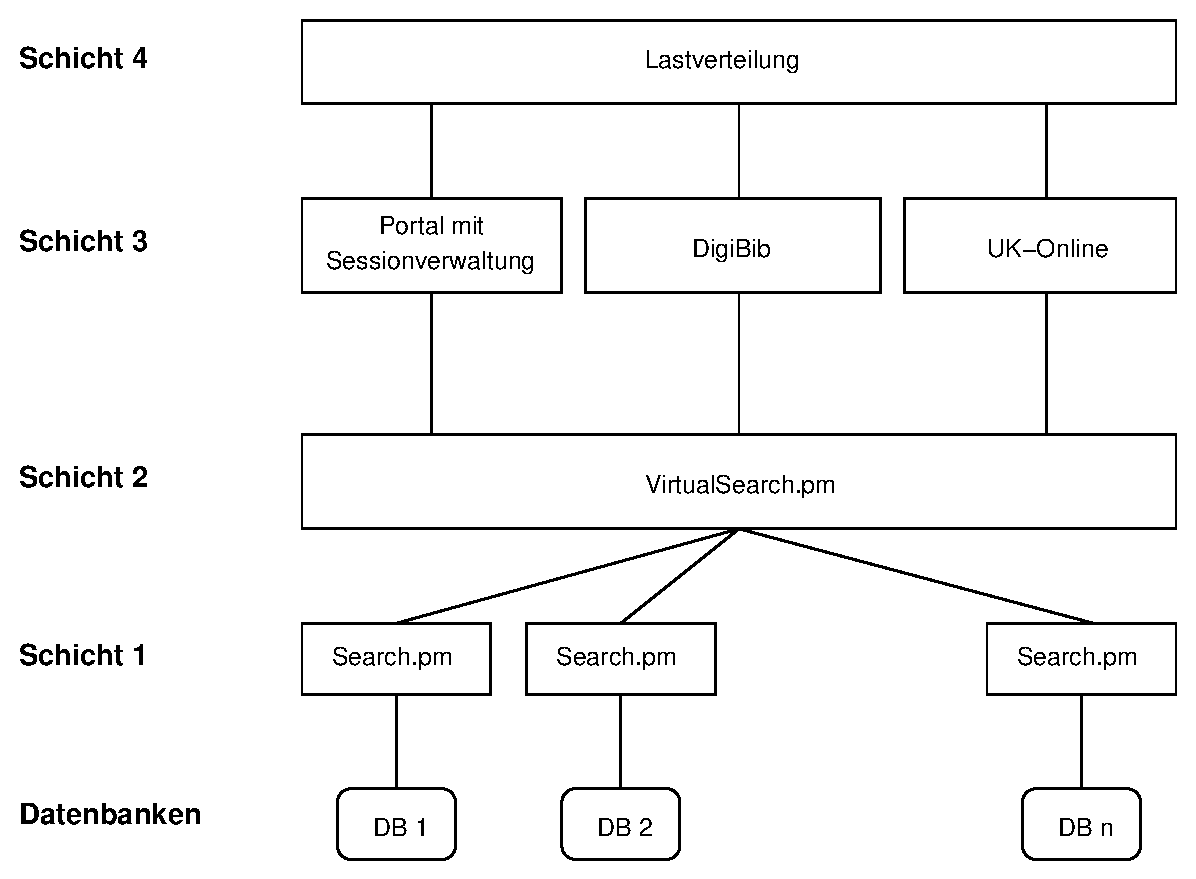
\includegraphics[width=12cm]{schicht04.eps}
    \end{minipage}
    \caption{Generelle Architektur der OpenBib-Portal-Suite}
  \label{bild:architektur}
  \vspace{3mm}
\end{shadowenv}
\end{figure}

\section{Die datenbankabhängige Schicht 1 -- \texttt{OpenBib::Search}}

In der untersten, der datenbankabhängigen Schicht greift das
Perl-Modul \texttt{OpenBib::Search} auf eine feste Datenbank zu.
Welche Datenbank dies ist, kann als Aufrufparamter dem Programm
mitgegeben werden. Dadurch ist es möglich, das gleiche Programm für
Recherchen über ver\-schie\-de\-ne Daten\-banken zu nutzen. Das Modul
selbst -- wie auch alle anderen unter
\begin{verbatim}
openbib/portal/perl/modules
\end{verbatim}
angesiedelten Module -- ist als Erweiterung des Apache-Webservers via
\texttt{mod\_perl} realisiert.  Dadurch arbeitet es außer\-ordentlich
schnell.


\section{Die datenbankübergreifende Recherche-Schicht 2 -- \texttt{OpenBib::VirtualSearch}}

Die datenbankübergreifende Recherche geschieht in der über
\texttt{OpenBib::Search} liegenden Schicht 2 (vgl. Abb.
\ref{bild:architektur}) mit dem Perl-Modul
\texttt{OpenBib::VirtualSearch}. Aufgabe dieses Modules ist es, eine
Suchanfrage und eine Anzahl an Recherche-Datenbanken vom Benutzer
entgegen\-zuneh\-men und genau diese eine Suchanfrage sequentiell an
jede der übergebenen Datenbanken zu schicken. Zu diesem Zweck werden
entsprechende Utility-Routinen aus dem im
\texttt{OpenBib::Search}-Kontext angesiedelten Modul
\texttt{OpenBib::Search::Util} verwendet.

Die Ergebnisse der einzelnen Recherchen werden entgegengenommen und in
Listenform auf\-be\-rei\-tet. Die jeweiligen Titel selbst sind in dieser
Gesamttrefferliste via URL mit einer Suchanfrage für genau diesen
Einzeltreffer mit \texttt{OpenBib::Search} verknüpft. 
Bei der
Auswahl eines einzelnen Treffers wird dadurch direkt in die
zugehörige Datenbank via \texttt{OpenBib::Search} gesprungen. 

Alle 'normalen' Verknüpfungs-Links (Normdaten, Hierarchien, etc.)
beziehen sich -- wir befinden uns nach der Auswahl eines Treffer wieder in
Schicht 1 -- auf genau diese eine Datenbank. Über das große
stilisierte 'G' bei den Normdaten kann jedoch auch an dieser Stelle
wieder eine datenbankübergreifende Recherche nach genau dem
zugehörigen Begriff gestartet werden. Der Benutzer hat somit bei
einem Einzeltreffer immer die Möglichkeit selbst zu entscheiden, ob
er sich bzgl. der Normdaten weiter im zugehörigen Katalog aufhalten
möchte, oder katalogübergreifend Recherchieren möchte.

Da in jedem Katalog die Verknüpfungen bereits in der Datenbank
existieren, ist ein 'sich treiben lassen' in einem festen Katalog
außer\-ordentlich schnell, während bei einer katalogübergreifenden
Suche ein kleiner Tribut zu zahlen ist, da nun effektiv wieder alle
Datenbanken mit einer 'neuen Suche' abgefragt werden.

Da \texttt{OpenBib::VirtualSearch} letztlich für die
datenbankübergreifende Gewinnung der Recherche\-er\-geb\-nisse
zuständig ist, werden nach erfolgreicher Recherche die Ergebnisse
aufgeteilt nach den einzelnen Katalogen in der Session-Datenbank
\texttt{session} 'gecached'. Durch das Caching der
Re\-cher\-che\-ergebnisse kann im Kontext von der Portal-Schicht 3
üeber das dort angesiedelte Modul \texttt{OpenBib::ResultLists} auch
eine Trefferlistenfunktionalität geleistet werden, in der man über
die Ergebnisse der letzten Recherche hinaus auch noch direkt auf die
Ergebnisse jeder zuvor eingegebenen Suche in der aktuellen Session
zugreifen kann.

\section{Die Portal-Schicht 3 mit weiteren externen Zugriffmechanismen}

\subsection{Das Portal mit Session- und Benutzerverwaltung}

In der Portalschicht wird dem Benutzer sessionbasiert in einer aus
zwei Frames bestehenden Web-Seite eine Arbeits- und Recherche-Oberfläche
geliefert. 

Der Einsprung-URL in das Portal wird durch das Modul
\texttt{OpenBib::StartOpac} realisiert.

Das Modul \texttt{OpenBib::StartOpac} kann über verschiedene
Parameter gesteuert werden, die z.B. für den direkten Sprung zu einem
einzelnen Treffer einer Datenbank oder der Anzeige einer
katalogeigenen Sicht des Portals Verwendung finden und gegebenenfalls
an nachgelagerte Module durchgereicht werden. Seine wesentliche
Aufgabe ist jedoch, eine eindeutige Session-ID zu generieren sowie ein
Frameset mit zwei Frames bereitzustellen.  Das obere Frame für die
Navigation wird durch das Modul \texttt{OpenBib::HeaderFrame}
gefüllt, das untere Frame standardmäßig zuerst durch das Modul
\texttt{OpenBib::SearchFrame}, das dem Navigations-Element 'Einfache
Recherche' bzw. 'Komplexe Recherche' entspricht.

Das Modul \texttt{OpenBib::HeaderFrame} ist für die Navigation im Portal
inklusive Counter für die Merkliste zuständig.

In der Navigation werden folgende Funktionalitäten angeboten:

\begin{description}
\item[Katalogauswahl] Die Auswahl der zu durchsuchenden Kataloge geschieht
  über eine entsprechende Aus\-wahl\-seite, die durch das Modul
  \texttt{OpenBib::DatabaseChoice} generiert wird.
\item[Recherche] Die Recherche-Maske wird über einen Aufruf von
  \texttt{OpenBib::SearchFrame} dargestellt.
\item[Trefferliste] Ein Zugriff auf Trefferlisten aus vorangegangenen
  Recherchen geschieht über das Modul \texttt{OpenBib::ResultLists},
  welches neben der verteilten Recherche auch für ein Caching der
  Ergebnis-Daten zuständig ist.
\item[Merkliste] Die Anzeige, Organisation sowie der Mailversand der
  Merkliste wird durch die Module
  \texttt{OpenBib::ManageCollection} und \texttt{OpenBib::MailCollection}
  über\-nom\-men. Bei Auswahl eines Treffers für die Merkliste wird
  \texttt{OpenBib::HeaderFrame} aktualisiert, und zeigt die neue Zahl
  gemerkter Treffer an.
\item[RSS] Über das Modul \texttt{OpenBib::RSSFrame} wird eine zu
  diesem View zugeordnete Liste an RSS-Feeds für die letzten 50
  Neuaufnahmen der entsprechenden Kataloge ausgegeben.
\item[Mein OpenBib] Über das Modul \texttt{OpenBib::Login}
  kann sich der Benutzer am Portal authentifizieren und so von
  weiteren personalisierten Funktionalitäten profitieren. Dazu
  gehören neben generellen Benutzereinstellungen
  (\texttt{OpenBib::UserPrefs}) u.a. per\-sis\-ten\-te Merklisten sowie
  Datenbankprofile (\texttt{OpenBib::DatabaseProfile}).

  Das Modul gewährt dabei den Zugang auf Grundlage seiner eigenen
  Datenbank, die über das Modul \texttt{OpenBib::SelfReg} via
  Selbstregistierung gefüllt wird, bzw. auf Grundlage von lokalen
  Bibliothekssystemen -- hier wird konkret das Bibliothekssystem Sisis
  SunRise unterstützt --, die über eine selbst entwicklte
  WebServices-Schnittstelle OLWS (Open Library WebServices)
  angesprochen werden können. Falls ein Benutzer sein
  selbstregistriertes Passwort vergessen hat, so kann er es sich über
  das Modul \texttt{OpenBib::MailPassword} per Mail zusenden lassen.
\item[Hilfe] Die Hilfeseite wird direkt als URL
  \texttt{/suchhilfe.html} angesprochen.
\item[Sitzung beenden] Beim Ende der Sitzung wird zum Modul
  \texttt{OpenBib::Leave} gesprungen, welches die sessionrelevanten Daten
  entfernt sowie einen URL in die Schicht 4 zur Lastver\-teilungs\-instanz
  \texttt{OpenBib::LoadBalancer} mit Angabe eines eventuell aktiven Views
  (Institutssicht) für einen er\-neu\-ten Einstieg in das Such-Portal
  bereitstellt.

\end{description}

\subsection{Externe Anbindung an die DigiBib}

Neben der Bereitstellung einer Recherche- und Arbeitsoberfläche für
den Endbenutzer, besteht auch die Möglichkeit über eine externe
Zugriffs-Schnittstelle automatisiert auf den Gesamtkatalog
zuzugreifen.

Eine solche Möglichkeit besteht in der Einbindung in das Such-Portal
\textbf{Digitale Bibliothek NRW} (DigiBib) des
Hoch\-schul\-bibliotheks\-zentrum NRW (hbz). Das Suchinterface besteht aus
einem fest definierten Such-URL und einem fest definierten
HTML-basierten Antwortformat für die Treffer. Grundsätzlich wird auf
eine Rechercheanfrage, z.B. unter Angabe eines Suchbegriffes für den
Titel, mit einer Kurztitelliste geantwortet. Es kann bestimmt werden,
welcher Teil der Kurztitelliste von den OpenBib-Daten\-banken
angefordert werden darf (Blätterfunktion mit frei wählbarem Offset
und Schrittweite). Darüber hinaus wird neben der Kurztitelliste auch
die Anzeige eines Einzeltreffers mit weiter\-gehen\-den Kategorien
angeboten. In der Kurztitelliste sind alle Informationen vorhanden, um
den Einzeltreffer aufzurufen.

\subsection{Externe Anbindung an UK-Online}

Eine weitere Anbindung besteht in das Universitätsportal UK-Online
von Herrn Prof. Lohnstein aus der Philosophischen Fakultät der
Universität zu Köln. Hier wird in UK-Online die Möglichkeit
angeboten eigenen Bibliographie-Listen zu verwalten. Der Aufbau einer
solchen Bibliographie-Liste geschieht über die Recherche in OpenBib
und anschließende Umwandlung und Ab\-spei\-cherung in ein
Bibliographie-Listen-Format.

Nach dem derzeitigen Stand sind beide externen Anbindung noch nicht in
einer lastverteilten Variante verfügbar. Diese ist jedoch kurz vor
der Fertigstellung.

\section{Die Lastverteilungs-Schicht 4}

Die Lastverteilungs-Schicht ist der erste Anlaufpunkt für die
Benutzung von OpenBib. Diese Schicht wird für das Portal durch das
Modul \texttt{OpenBib::LoadBalancer} und \texttt{OpenBib::ServerLoad} gebildet.
Entscheidungsgrundlage für die Verteilung ist die Auslastung der
betroffenen Recher, deren generelle Ansprechbarkeit sowie die
generelle Funktionsfähigkeit des MySQL-Daten\-bank\-sys\-tems.

Durch diese vorgeschaltete Verteilung der Recherche-Sitzungen auf
mehrere Rechner ergeben sich mehrere Vorteile:

\begin{enumerate}
\item Es wird eine Lastverteilung durchgeführt. Wenn also ein Nutzer
  einen dieser URL's aufruft, so wird er auf den Rechner
  weitergeleitet, der am wenigsten belastet ist.  Dies ist primärer
  Zweck dieser Schicht.
\item Ist ein Rechner defekt -- im Sinne von 'nicht ansprechbar'
  bzw. 'DBMS-seitig nicht funk\-tions\-fä\-hig' --, dann wird er bei der
  Verteilung/Weiterleitung nicht mehr berücksichtigt und die Benutzer
  werden nur noch auf die verbliebenen Rechner verteilt. In diesem
  Fall ist bei der Weiterleitung mit einer kurzen Wartezeit von
  maximal 5 Sekunden (Timeout) zu rechnen.  Automatisch wird
  zusätzlich an den Administrator eine Mail ge\-ne\-riert, die ihn
  auf den defekten Rechner hinweist. Ein Sonderfall ist natürlich der
  'Verteilungs\-rech\-ner' selbst, bei dessen Ableben temporär ein
  anderer Rechner unter seiner Identität einspringen muß. Letzteres
  kann selbstverständlich nicht automatisch geschehen und muss
  manuell konfiguriert werden. In diesem Sinn besteht mit dem
  Lastverteilungsrechner ein Singe-Point-Of-Failure, der nur über
  HA-Mechanismen ausgeräumt werden kann.
\item Werden Wartungsarbeiten auf einem der Rechner ausgeführt, so
  kann man ihn selbst temporär aus der Verteilung/Weiterleitung
  herausnehmen. Auf diese Weise ändert sich für die Nutzer nichts,
  es werden dann die verbliebenen Rechner verwendet.
\end{enumerate}


\chapter{Konzepte und Interna von OpenBib}


\section{Datenbankstruktur}

Die bibliographischen Daten verteilen sich auf eine festgelegte Weise
auf verschiedene Tabellen. Es sind dies die Tabellen der
\textbf{Normdaten}, der \textbf{Verknüpfungen}, der \textbf{Anfangssuche}
sowie der \textbf{zwischengespeicherten Kurztreffer}.


\subsection{Normdaten}

Es gibt 6 Normdatenbereiche. Es sind dies
\begin{enumerate}
\item Reine Titeldaten
\item Verfasser bzw. Personen
\item Körperschaften bzw. Urheber
\item Schlagworte
\item Notationen bzw. Systematik
\item Exemplare
\end{enumerate}

Intern ist jedem dieser Bereiche ein alphabetisches sowie ein
numerisches Kürzel zugeordnet. Für die Mehrsprachigkeit
(Internationalisierung / I18N) wird darüber hinaus vor der vierstelligen
Kategorienummer ein Prefix verwendet. Das alphabetische Kürzel ist
Teil des Tabellen\-namens, das numerische Kürzel wird zur
Kennzeichnung des Normdatentyps in der Verknüpfungs\-tabelle
\texttt{conn} (s.u.)  verwendet.

\begin{table}
  \begin{shadowenv}
    \vspace{3mm}
    \begin{center}
      \begin{tabular}[c]{lccc}
        Normdatentyp   & alphabet. Kürzel & numer. Kürzel & I18N-Prefix\\
        \hline
        Titel          & tit              & 1             & T\\
        Verfasser      & aut              & 2             & P\\
        Körperschaften & kor              & 3             & C\\
        Schlagworte    & swt              & 4             & S\\
        Notationen     & notation         & 5             & N\\
        Exemplare      & mex              & 6             & X\\
      \end{tabular}
    \end{center}
    \caption{Normdatentypen mit Kürzeln und I18N-Prefix\label{normkuerzprefix}}
    \vspace{3mm}
  \end{shadowenv}
\end{table}

Jedem Normdatentyp sind drei Tabellen zugeordnet, deren Grundname
dem alphabetischen Kürzel entspricht.

\begin{description}
\item[Darstellung] In der Tabelle, die dem alphabet. Kürzel
  entspricht, werden die Kategorien mit ihren Inhalten abgelegt. Die
  Inhalte sind UTF8-kodiert und werden so 1:1 ausgegeben. Diese
  Tabellen heissen \texttt{tit}, \texttt{aut}, \texttt{kor},
  \texttt{notation}, \texttt{swt} sowie \texttt{mex}.
\item[Wortanfangssuche] Der ersten, primär für die Darstellung
  zuständigen Tabelle, ist eine zweite zugeordnet, über die String-
  oder Wortanfangssuchen realisiert werden können. Der Tabellen\-name
  besteht aus dem alphabet. Kürzer, an das \texttt{\_string} angehängt
  ist. Der Inhalt in diesen Tabellen wurde bereits auf seine Grundform
  reduziert. Welche Kategorien in diese Tabellen wandern, lässt sich
  generell sowie für einzelne Katalog konfigurieren. Die Namen dieser
  Tabellen heissen \texttt{tit\_string}, \texttt{aut\_string},
  \texttt{kor\_string}, \texttt{notation\_string},
  \texttt{swt\_string} sowie \texttt{mex\_string}.
\item[Volltextsuche] Der ersten, primär für die Darstellung
  zuständigen Tabelle, ist eine weitere dritte zugeordnet, über die
  Volltextsuchen realisiert werden können. Der Tabellen\-name besteht
  aus dem alphabet. Kürzer, an das \texttt{\_ft} -- wie fulltext --
  angehängt ist. Der Inhalt in diesen Tabellen wurde bereits auf seine
  Grundform reduziert. Welche Kategorien in diese Tabellen wandern,
  lässt sich generell sowie für einzelne Katalog konfigurieren. Die
  Namen dieser Tabellen heissen \texttt{tit\_ft}, \texttt{aut\_ft},
  \texttt{kor\_ft}, \texttt{notation\_ft}, \texttt{swt\_ft} sowie
  \texttt{mex\_ft}.
\end{description}

\subsection{Verknüpfungen}

Um einen vollständigen bibliographischen Titelsatz zu erhalten müssen
die jeweiligen Kategorien aus den einzelnen Normdaten-Tabellen über
entsprechende Verknüpfungen in der Tabelle \texttt{conn} einander
zugeordnet werden. Ausgehend von einer ID in einer Normdaten-Tabelle
-- typischerweise \texttt{tit} -- wird eine ID aus einer anderen (bei
hierarchischen Titelverknüpfungen auch der gleichen) Normdaten-Tabelle
zugeordnet.

Über die \emph{Zusammenführung zu einem vollständigen bibliographischen
Titelsatz} hinaus wird über diese Tabelle die \emph{Navigation zwischen
  einzelnen Titeln} über die jeweiligen Normdaten-ID's realisiert.

Im Falle der Zusammenführung zu einem bibliographisch vollständigen
Titelsatz kann in \texttt{conn} zusätzlich definiert werden,
welche Kategorie der Inhalt aus der jeweilig anderen Normdatei im
Titelsatz bekommen soll (\texttt{category}) und ob eine
Zusatzinformation (\texttt{supplement}) -- z.B. \texttt{Hrsg.} --
bezogen auf den speziellen Titel zu dem verknüpften Normdateninhalt
(z.B.  \texttt{aut}) hinzugefügt werden soll.

Im Falle hierarchischer Werke -- damit sind sowohl \texttt{sourcetype}
wie auch \texttt{targettype} gleich 1 (Titel), ist sofort ersichtlich,
dass

\begin{itemize}
\item wenn die lokale Titelsatz-ID im \texttt{targettype} auftritt,
  die Titelsatz-ID im \texttt{sourcetype} demnach die ID des
  \textbf{untergeordneten} Titelsatzes ist, während
\item wenn die lokale Titelsatz-ID im \texttt{sourcetype} auftritt,
  die Titelsatz-ID im \texttt{targettype} demnach die ID des
  \textbf{übergeordneten} Titelsatzes ist.
\end{itemize}


\subsection{Zwischengespeicherte Kurztreffer}

Zur Beschleunigung der Informationsbestimmung für einen Kurztreffer
werden in der Tabelle \texttt{titlistitem} die jeweiligen
Kategorie-Inhalte bereits in der Form eines Caches abgelegt. Damit
müssen die Informationen nicht aus allen Normdaten-Tabellen unter
Zuhilfenahme der Ver\-knüp\-fungs\-tabelle bestimmt werden, sondern stehen
direkt zur Verfügung.

\subsection{Anfangssuche}


Grundsätzlich werden zwei Suchtypen genutzt. Wenn ein Nutzer seine
Suchanfrage eingibt, dann wird für diese Anfangssuche zunächst in
einem von zwei Recherche-Backends recherchiert. Die Backends lassen sich
augrund der moduleren Struktur von OpenBib sehr einfach erweitern.

Mögliche Recherche-Backends sind 

\begin{description}
\item[SQL] In der Tabelle \texttt{search} wird entsprechend der
  \emph{eingegebenen Suchanfrage} recherchiert und eine Liste
  zutreffender Titel-ID's zurückgeliefert. Mit diesen Titel-ID's
  wird dann entweder aus den Normdatentabellen oder der Tabelle
  \texttt{titlistitem} der
  zwischengespeicherten Kurz\-treffer  eine Liste
  von Kurzreffern für die Anzeige bestimmt.
\item[Xapian] Alternativ zur Suche via SQL kann auf die
  Suchmaschinen-Technologie von Xapian zurückgegriffen werden. Es wird
  dann die eingegebene Suchanfrage in dem entsprechenden Xapian-Index
  recherchiert. Zurückgeliefert wird eine Liste der direkt im
  Xapian-Index abgespeicherter Kurztreffereinträge, die für die
  Anzeige bestimmt sind
\end{description}

Nach diesen zwei Varianten der Anfangssuche wurde dem Nutzer eine
Liste von Kurztitelaufnahmen präsentiert, von denen dann direkt in die
SQL-Datenbank zu einem vollständigen Treffer in einem spezifischen
Katalog gesprungen werden kann.

Ist man erst einmal in einem Treffer eines einzelnen Katalogs, dann
wird dort primär mit der Verknüpfungstabelle \texttt{conn} über die
Normdaten navigiert. Darüber hinaus kann von hier aber auch wieder eine
globale Anfangssuche über eines der beiden Recherche-Backends angestossen
werden.


\section{Kategorienformat}
\subsection{Allgemeine Informationen}
Die bibliographische Datenhaltung in der MySQL-Datenbank ist
grundsätzlich unabhängig vom verwendeten Kategorienschema. Damit
können dort -- ohne Änderung oder Erweiterung der Datenbank --
beliebige andere Kategorien, als die aus dem an den MAB2-Standard angelehnte
Standardkategorien\-schema, abgelegt und verarbeitet werden.

Eine Kategorie in der bibliographischen Datenbank zeichnet sich durch
folgendes aus:

\begin{itemize}
\item Eine Kategorie gehört zu einem Normdatentyp. Mögliche
  Normdatentypen sind Titel (tit, \textbf{T}, \texttt{1}), Verfasser
  bzw. Person (aut, \textbf{P}, \texttt{2}), Körperschaft bzw. Urheber
  (kor, \textbf{C}, \texttt{3}), Schlagworte (swt, \textbf{S},
  \texttt{4}), Systematik bzw. Notation (notaton, \textbf{N},
  \texttt{5}) und Exemplare (mex, \textbf{X}, \texttt{6}).
\item Eine Kategorie besteht aus der numerischen ID bezogen auf einen
  Normdatentyp, einer Kategorienummer, einem numerischen
  Indikator\footnote{Mit dem numerischen Indikator können entweder
    alphabetische Indikatoren gemappt werden (a gleich 1, b gleich 2
    usw.), eine Multiplizität der Kategorie ausgedrückt werden (1.
    Exemplar gleich 1, 2. Exemplar gleich 2) oder auch beides zusammen
    über Modulos (a des 1. Exemplars gleich 1, b des 1. Exemplars
    gleich 2, a des 2. Exemplars gleich 3, b des 2. Exemplars gleich
    4)}.
\item Jeder Kategorie ist ein abstrakter Bezeichner zugeordnet, dem
  wiederum pro Sprache ein Beschreibungstext zugeordnet werden
  kann. Pro Datenbank können bei Bedarf andere Beschreibungstexte
  zugeordnet werden
\end{itemize}


\subsection{Internationalisierung}


\subsubsection{Standardmechanismus}

Um Kategoriebezeichnungen für die Ausgabe mehrsprachig aufbereiten zu
können, werden aus den Kategoriennummern internationalisierbare
Kategoriebezeichner für \texttt{GNU gettext} gebildet. Dazu wird der
auf vier Stellen vorgenullten Kategorienummer der Normdatenprefix
vorangestellt (vgl. Abb. \ref{normkuerzprefix}).

Das Bezeichner-Format ist damit:

\begin{verbatim}
<Normdaten I18N-Prefix><4-stellige Kategorienr.>
\end{verbatim}

Der Bezeichner für die Kategorie \texttt{331} (HST) in den Titelnormdaten
lautet demnach \texttt{T0331} und der Bezeichner für die Kategorie
\texttt{1} in den Verfassernormdaten (Ansetzungsform) entsprechend
\texttt{P0001}.

Damit ergibt sich folgende Abhängigkeit:

\begin{verbatim}
Kategorie-Nr. (331) -> Kategorie-Bezeichner (T0331) 
                    -> Kategorieausgabebezeichnung ('HST')
\end{verbatim}

Damit die einzelnen Kategorie-Bezeichner automatisiert mit dem
Programm \texttt{xgettext.pl} erkannt und in die I18N-Message-Kataloge
übertragen werden können, werden sie in den jeweiligen Templates an
den Stellen als Kommentar aufgeführt, an denen definiert wird, welche
Kategorien in welcher Reihenfolge angezeit werden sollen. In diesen
Kommentaren sind sie in einem \texttt{maketext}-Aufruf gekapselt.

Als Beispiel wird das Template \texttt{visible\_categories\_titset}
betrachtet:

\begin{verbatim}
[%# Ausgabekategorien %]
[% categories = [
                'T0100', # msg.maketext("T0100") Verfasser
                'T0101', # msg.maketext("T0101") Person
                'T0103', # msg.maketext("T0103") Gefeierte Person
                'T0200', # msg.maketext("T0200") Urheber
                'T0201', # msg.maketext("T0201") Koerperschaft
                'T0089', # msg.maketext("T0089") Bandangabe  
...
\end{verbatim}

Der für die Internationalisierung wesentliche Teil -- der benötigt
wird -- ist

\begin{verbatim}
# msg.maketext("T1234")
\end{verbatim}

\subsubsection{Katalogweise Umbenennung der Kategoriebezeichnungen}

Es gibt Situationen in denen es zwingend notwendig wird für eine
Kategorie-Nr. in einer ganz speziellen Datenbank eine andere
Kategorieausgabe\-bezeichung zu verwenden -- und diese
selbst\-verständlich mehrsprachig.

Ausgehend von einer Kategorie in der Datenbank -- z.B. 331 -- wird
dafür ein \emph{Virtueller Kategorie-Bezeichner} gebildet, der
zusätzlich zum bereits bekannten Bezeichner -- mit Bindestrich
getrennt -- den Datenbanknamen angehängt hat. Das Bezeicher-Format ist
dann

\begin{verbatim}
<Normdaten I18N-Prefix><4-stellige Kategorienr.>-<DB-Name>
\end{verbatim}

Soll die Kategorieausgabebezeichnung z.B. für die Kategorie
\texttt{331} in der Datenbank \texttt{test} auf \texttt{Titel}
geändert werden, so wird hierfür der virtuelle Bezeichner
\texttt{T0331-test} verwendet, der so in die Message-Kataloge mit der
Ausgabebezeichnung \texttt{Titel} Eingang findet. Dieses Beispiel wäre
in der Realität selbst\-verständlich recht sinnlos.

Vorteil dieses Mechanismus ist, daß unter Beibehaltung des internen --
sinnvollerweise einheitlichen -- Kategorienschemas für einzelne
Kataloge die Kategorieausgabebezeichnung individuell angepasst werden
kann.

Damit dieser Mechanismus greifen kann müssen jedoch folgende
Vorarbeiten erfolgen:

\begin{description}
\item[Kennzeichnung der Kategorien] Die Kategorien, die für eine
  Datenbank 'umettikettiert' werden sollen, müssen für die
  entsprechende Datenbank in dem Modul \texttt{OpenBib::Config.pm}
  unter \texttt{categorymapping} definiert werden.

  Im \texttt{Titel}-Beispiel würde dieser Eintrag wie folgt aussehen:
  
\begin{verbatim}
# Katalogabhaengige Kategorie-Mappings

categorymapping => {

      test => {
                'T0331' => 1,
              },

},
\end{verbatim}


\item[Anpassung des Templates] Für die Nutzung der neuen virtuellen
  Kategorie-Bezeichner im Template muß zunächst ein entsprechendes Fragment
  hinzugefügt werden:

\begin{verbatim}
# Nachgeschaltete datenbankspezifische Kategorienamen-Mappings sind
# in Config.pm fuer die entsprechende Datenbank definiert
# und werden im Message-Katalog als <Kategorie>-<Datenbankname>
# kodiert.
IF config.categorymapping.$database.$category ;
   thiscategory = "${category}-${normset.database}" ;
ELSE ;
   thiscategory = ${category} ;
END;
\end{verbatim}

  Darüber hinaus sollten für die automatische Extraktion der
  I18N-Bezeichner über das Hilfs\-programm \texttt{xgettext.pl} in den Kommentaren des
  Templates \texttt{visible\_categories\_titset} die neuen virutellen
  Kategorie-Bezeichner genannt werden:

\begin{verbatim}
'T0331', # msg.maketext("T0331-test") Titel
\end{verbatim}

  Auch hier ist der wesentliche Teil des Kommentars:

\begin{verbatim}
msg.maketext("T0331-test")
\end{verbatim}

\end{description}
\subsection{Beispiel}

Als Beispiel verwenden wir die Titelaufnahme des Hauptaufnahme des
mehrbändigen Werkes \emph{TCP/IP Illustrated} von \emph{Richard W.
  Stevens}. Diese Titelaufnahme sieht wie folgt aus:

\begin{table}
  \begin{shadowenv}
    \vspace{3mm}
    \begin{center}
      \begin{tabular}{ll}
        id	        & 5899\\
        Verfasser	& Stevens, W. R.\\
        HST	        & TCP/IP Illustrated\\
        Vorl.Verfasser	& W. Richard Stevens\\
        Verlagsort	& Reading, Mass. [u.a.]\\
        Verlag	        & Addison-Wesley\\
        Schlagwort	& TCP / IP\\
        Schlagwort	& Internet\\
        Schlagwort	& Kommunikationsprotokoll\\
        Unterordnungen	& 2\\
      \end{tabular}
    \end{center}
    \caption{Beispiel-Titel\label{beispieltitel}}
    \vspace{3mm}
  \end{shadowenv}
\end{table}

\subsubsection{Verknüpfungen}
Dieser Titel verteilt sich nun mit seinen Daten auf mehrere
Normdaten-Tabellen. Es sind dies hier konkret die Titeltabelle
\texttt{tit}, die Verfassertabelle \texttt{aut}, die Schlagworttabelle
\texttt{swt} sowie für die Verknüpfungen des Titelsatzes mit den
anderen Normdaten und die Abhängigkeiten zwischen Titeln
(Unterordnungen) die Verknüpfungstabelle \texttt{conn}.

Zunächst werden für diesen Titel die Informationen in der
Titelnormdaten-Tabelle dargestellt mit 

\begin{verbatim}
mysql> select * from tit where id=5899;
\end{verbatim}

dargestellt.

\begin{verbatim}
+------+----------+-----------+-----------------------+
| id   | category | indicator | content               |
+------+----------+-----------+-----------------------+
| 5899 |        1 |         0 | 05899                 |
| 5899 |        2 |         0 | 27.05.2003            |
| 5899 |      331 |         1 | TCP/IP Illustrated    |
| 5899 |      359 |         1 | W. Richard Stevens    |
| 5899 |      410 |         1 | Reading, Mass. [u.a.] |
| 5899 |      412 |         1 | Addison-Wesley        |
+------+----------+-----------+-----------------------+
6 rows in set (0.30 sec)
\end{verbatim}

Dieser Titelsatz ist mit den anderen Normdaten verknüpft. Die ID's der
verknüpften Sätze erhält man mit

\begin{verbatim}
mysql> select * from conn where    (sourceid=5899 and sourcetype=1) 
                                or (targetid=5899 and targettype=1);
\end{verbatim}

zu:

\begin{verbatim}
+----------+----------+------------+----------+------------+------------+
| category | sourceid | sourcetype | targetid | targettype | supplement |
+----------+----------+------------+----------+------------+------------+
|      100 |     5899 |          1 |      684 |          2 |            |
|      710 |     5899 |          1 |      133 |          4 |            |
|      710 |     5899 |          1 |      604 |          4 |            |
|      710 |     5899 |          1 |      571 |          4 |            |
|        0 |     5900 |          1 |     5899 |          1 |            |
|        0 |     5901 |          1 |     5899 |          1 |            |
+----------+----------+------------+----------+------------+------------+
6 rows in set (0.11 sec)
\end{verbatim}

Es ist damit ersichtlich, dass 

\begin{itemize}
\item der Verfasser des Titels (\texttt{category:100}, \texttt{targettype:2}) die ID \texttt{684} hat
\item die drei Schlagworte des Titels (\texttt{category:710)}) die ID's
  \texttt{133}, \texttt{604} sowie \texttt{571} haben
\item Die Unterordnungen des Titels (\texttt{sourceid}) die Titel-ID's
  \texttt{5900} und \texttt{5901} haben.
\end{itemize}

Damit ergibt sich der Verfasser mit

\begin{verbatim}
mysql> select * from aut where id=684;
\end{verbatim}

zu 

\begin{verbatim}
+-----+----------+-----------+---------------------+
| id  | category | indicator | content             |
+-----+----------+-----------+---------------------+
| 684 |        1 |         0 | Stevens, W. R.      |
| 684 |      102 |         1 | Stevens, W. Richard |
+-----+----------+-----------+---------------------+
2 rows in set (0.04 sec)
\end{verbatim}

sowie die Schlagworte mit 

\begin{verbatim}
mysql> select * from swt where id in (133,604,571);
\end{verbatim}
zu

\begin{verbatim}
+-----+----------+-----------+-----------------------------------------------+
| id  | category | indicator | content                                       |
+-----+----------+-----------+-----------------------------------------------+
| 133 |        1 |         1 | TCP / IP                                      |
| 133 |      113 |         1 | Kommunikationsprotokoll                       |
| 133 |      108 |         1 | 30m                                           |
| 133 |      102 |         1 | Transmission control protocol / Internet pr...|

| 571 |        1 |         1 | Kommunikationsprotokoll                       |
| 571 |      108 |         1 | 30                                            |
| 571 |      102 |         3 | Kommunikationstechnik                         |
| 571 |      102 |         2 | Datenübertragung                              |
| 571 |      102 |         1 | Übertragungsprotokoll                         |

| 604 |        1 |         1 | Internet                                      |
| 604 |      108 |         1 | 30m                                           |
| 604 |      102 |         2 | TCP / IP / Internetzwerk                      |
| 604 |      102 |         1 | Internetzwerk / TCP / IP                      |
+-----+----------+-----------+-----------------------------------------------+
\end{verbatim}

Für die untergeordneten Titel wiederholt sich diese gesamt Prozedur
mit den zwei Titel-ID's \texttt{5900} und \texttt{5901}.

\subsubsection{Internationalisierung}

Für die Internationalisierung der Bezeichnungstexte wird für die
einzelnen Titelkategorien ein Bezeichner durch Vornullen der
Kategorienummer auf 4 Stellen sowie Voranstellen des Normdatenkürzels.

Damit erhält man für den Titel folgende Bezeichner

\begin{description}
\item[T0100] Aus der Kategorie \texttt{100} von \texttt{conn}
\item[T0331] Aus der Kategorie \texttt{331} von \texttt{tit}
\item[T0359] Aus der Kategorie \texttt{359} von \texttt{tit}
\item[T0410] Aus der Kategorie \texttt{410} von \texttt{tit}
\item[T0412] Aus der Kategorie \texttt{412} von \texttt{tit}
\item[T0710] Aus der Kategorie \texttt{710} von \texttt{conn}
\item[T5000] Aus der Anzahl der Verweise in \texttt{conn}. Im
  Gegensatz zu den vorangegangenen MAB2-Kategorien wurde diese
  willkürlich zu \texttt{5000} definiert.
\end{description}


\section{Kaskadierungsmechanismus bei Templates und Stylesheets}

Ein wesentlicher Aspekt bei dem Einsatz und der alltäglichen Arbeit an
einer Portalsoftware ist der Aufwand, der zu leisten ist, wenn -- auf
Grundlage einer installierten Portalsoftwarebasis -- viele visuell
unterschiedliche Einzel-Portale erstellt und betreut werden müssen.

Einige Systeme bieten traditionell für ihr \emph{Standard-Portal} ein
abgeschlossenes Set an Templates, Stylesheets, Bilder oder JSP's an.
Beim Aufbau eines neuen \emph{Portals} muß dann selbst bei kleinsten
Unterschieden zum Standard-Set eben jenes vollständig geklont werden,
um dann für das neue Portal davon ausgehend vereinzelte Änderungen
vorzunehmen. Da damit dann aber pro Portal unterschiedlich geänderte
Klones des Standard-Sets existieren, resultiert daraus, dass pro
Portal nicht mehr sofort ersichtlich ist, wo genau Änderungen
vorgenommen und wo der Standard verwendet wurde.

Aus diversen Erfahrungen mit dieser Art an Systemen kann ich
konstatieren, daß der Aufbau, Betrieb und insbesondere die Updates bei
einem Versionswechsel in solchen Systemen ein Adminis\-tra\-tions-Albtraum
ist.

Aus diesen Erfahrungen ist ein alternatives Konzept entstanden, bei
dem ebenfalls ein Standard-Set definiert wird, dann jedoch durch Klonen
\emph{einzelner} abweichender Templates und Stylesheets -- und nicht
aller -- in fest definierte Verzeichnisse im Dateibaum die
Individualisierung für das jeweilige neue Portal erfolgt.

\emph{Grunsätzlich gilt: Existiert ein spezifischeres Template oder
Stylesheet gleichen Namens, so wird dieses verwendet und nicht das
Standard-Template.}


\subsection{Templates}

In OpenBib befindet sich der Standard-Set an Templates in dem
Verzeichnis, das in dem Modul \texttt{OpenBib::Config.pm} unter
\texttt{tt\_include\_path} definiert ist. Default ist das Verzeichnis
\begin{verbatim}
/opt/openbib/templates
\end{verbatim} 

In diesem Verzeichnis existieren zwei
spezielle Unterverzeichnisse, die für die Kaskadierung der Templates
wesentlich sind. Sie heissen \texttt{views} und \texttt{database}.

Eigenständige Portale werden in OpenBib als Views (Sichten)
definiert. Jeder View erhält einen Namen, unter dem er angesprochen
werden kann. Jedem View zugeordnet sind ferner verschiedene
Datenbanken, die beim Aufruf des Views vorausgewählt sind.

Anhand eines Beispiels soll nun demonstriert werden, wie für einen
neuen View \texttt{rheinlandbib} ein einziges Template --
\texttt{corporate\_banner} angepasst wird. In diesem Template werden
Logo-Texte und Graphiken des Views definiert.

Zunächst muß der entsprechende View in der Web-Administration erzeugt
werden. Dazu wird ihm dort ein Name -- hier \texttt{rheinlandbib} --,
eine Beschreibung, eine Aktivität (aktiv oder nicht) sowie
verschiedene Datenbanken zugeordnet.

Um nun unter Beibehaltung aller anderen Templates lediglich das
Template \texttt{corporate\_banner} für den neuen View zu
individualisieren, geht man wie folgt vor:

\begin{enumerate}
\item Man erzeugt im Unterverzeichnis \texttt{views} von
  \texttt{tt\_include\_path} ein neues Verzeichnis mit dem Namen des neuen
  Views -- hier \texttt{rheinlandbib}.
\item Man kopiert die zu ändernden Templates aus
  \texttt{tt\_include\_path} in das neue Verzeichnis -- hier \texttt{corporate\_banner}.
\item Man ändert das Template in dem neuen Verzeichnis.
\end{enumerate}

Damit ist der neue View bis auf das Template
\texttt{corporate\_banner} identisch mit der Standard-Darstellung des
Portals.

Diese Vorgehensweise hat neben der Einfachheit den entscheidenen
Vorteil, daß View-spezifische Template-Änderungen sehr geordnet in den
einzelnen View-spezifischen Verzeichnissen abgelebt sind. Dies schafft
Übersicht, Ordnung - und vereinfacht die weitergehende Administration
-- u.a. bei Updates -- erheblich.

Manchmal kann es auch notwendig werden, dass für eine spezielle
Datenbank eine vom Standard abweichende Einzeltitel-Darstellung
benötigt wird -- z.B. wenn Kategorie-Inhalte anders gruppiert werden
sollen\footnote{An der USB Köln war dies z.B. insbesondere für die
  Titeldarstellung der Digitalen Einbandsammlung wesentlich, da in
  dieser speziellen Sicht die Informationen nach Titel und Einband
  gruppiert werden mussten.}.

Die Vorgehensweise entspricht weitestgehend den bei den Views, nur daß
das datenbank-spezifische Unterverzeichnis nun \texttt{database} und
nicht \texttt{views} heisst, und dort die anzulegenden Verzeichnisse
den Namen der Datenbank tragen, für die entsprechende Templates
anzupassen waren, also

\begin{enumerate}
\item Man erzeugt im Unterverzeichnis \texttt{database} von
  \texttt{tt\_include\_path} ein neues Verzeichnis mit dem Namen der
  relevanten Datenbank -- hier \texttt{einbaende}.
\item Man kopiert die zu ändernden Templates aus
  \texttt{tt\_include\_path} in das neue Verzeichnis -- hier u.a. \texttt{search\_showtitset}.
\item Man ändert das Template in dem neuen Verzeichnis.
\end{enumerate}


\section{Internationalisierung}

\subsection{Allgemeine Informationen zu GNU gettext}

Zur Unterstützung von verschiedenen Sprachen durch das Portal wurde
auf \texttt{GNU gettext} zurück gegriffen, das eine \emph{best
  practice} in diesem Bereich darstellt und von unzähligen Projekten
und Programmen verwendet wird, wie z.B. den KDE-Projekt mit mehr als
40 unterstützten Sprachen.

\texttt{GNU gettext} zeichnet sich im Vergleich zu anderen Mechanismen
dadurch u.a. dadurch aus, daß in den Templates die einzelnen zu
übersetzenden Textbezeicher nicht numerisch sind, sondern aus
gewöhnlichem Text in einer Basis-Sprache -- typischerweise Englisch,
bei OpenBib bisher Deutsch -- bestehen. Damit ergeben sich
verschiedene Vorteile:

\begin{itemize}
\item Die Templates bleiben lesbar und beherrschbar. Bei numerischen
  Bezeichnern hingegen sieht man in einem Template gar nicht mehr, wo
  genau welcher Text steht.
\item Die eigentliche Übersetzung lässt sich an entsprechende
  Mitarbeiter auslagern, die weder um die Programmierung noch die
  Templates wissen müssen.
\end{itemize}

Weitere Vorteile von \texttt{GNU gettext} sind:

\begin{itemize}
\item Die Möglichkeit der Verwendung von Platzhaltern
\item Es existiert ein ganzes Toolset, um die Internationalisierung so
  automatisiert wie möglich durchzuführen. Gerade dies stellt einen
  hohen Wert dar.
\end{itemize}

\subsection{Technische Realisierung}

Während \texttt{GNU gettext} seine Wurzeln im Wesentlichen in der
\texttt{C}- und \texttt{C++}-Welt hat, wird in Perl sehr gerne
stattdessen \texttt{Maketext} verwendet, welches jedoch zwar
zusätzlich die gezielte Bildung von Pluralen mit \texttt{quant}
unterstützt, jedoch nicht über ein vergleichbares Toolset wie
\texttt{GNU gettext} verfügt.

OpenBib setzt zur Internationalisierung das Modul
\texttt{Locale::Maketext::Lexicon} von Audrey Tang ein, das sich auf
Perl-Seit wie \texttt{Maketext} verhält, im Backend jedoch speziell
\texttt{GNU gettext} einsetzt. Damit verwendet OpenBib das \emph{Beste
aus beiden Welten}.

Damit wird konkret in den Templates die \texttt{Maketext}-Syntax
verwendet, während die automatische Message-Tag-Extraktion aus den
Templates \texttt{GNU gettext}-Syntax liefert.

Um in einem Perl-Programm oder einem Template die
Text zu Internationalisieren geht man wie folgt vor:

\begin{description}
\item[Perl-Programm] Der Text wird mit einem Methodenaufruf
  \texttt{maketext} des Message-Objektes \texttt{\$msg}
  gekapselt. Letzeres wird in jedem \texttt{mod\_perl}-Handler über
  \texttt{OpenBib::L10N} instanziiert.

  Beispiel:

\begin{verbatim}
$msg->maketext("Ungültige Session")
\end{verbatim}

\item[Template] Der Text wird ebenfalls mit einem entsprechenden
  Methoden-Aufruf gekapselt -- diesmal jedoch in der
  Template-Toolkit-Syntax mit dem übergebenen Message-Objekt \texttt{\$msg}.

  Beispiel:

\begin{verbatim}
[% msg.maketext("Suchhistorie") %]
\end{verbatim}
\end{description}

Nachdem neue Begriffe so gekennzeichnet wurden oder andere geändert,
muß der Message-Katalog aktualisiert werden.

Dazu sind folgende Schritte notwendig:

\begin{enumerate}
\item Aktualisierung der Datei \texttt{portal/perl/locales/FILES}. Dort
  sind alle relevanten Datei\-namen aufgeführt, die
  übersetzt werden sollen.
\item Aufruf des mitgelieferten Hilfsprogramms
  \texttt{xgettext.pl}. Es werden damit aus allen in  \texttt{FILES}
  genannten Dateien die Message-Tags extrahiert und in einer Datei
  \texttt{message.po} abgelegt.
\item Abgleich von \texttt{message.po} mit dem bereits existierenden
  Message-Katalog -- \newline z.B. \texttt{de/LC\_MESSAGES/openbib.po}:

\begin{verbatim}
msgmerge -U de/LC_MESSAGES/openbib.po message.po
\end{verbatim}
\item Übersetzen der Sprachdatei \texttt{openbib.po} mit einem
  geeigneten Programm. Sehr zu empfehlen ist hier das KDE-Programm
  \texttt{kbabel}.
\end{enumerate}

Nach dem Restart des Apache-Daemons sind die Änderungen aktiv.

\section{Content-Enrichment}

\subsection{Hintergrund}

In NRW werden derzeit Scan-Projekte durchgeführt, in denen die
Inhaltsverzeichnisse von Büchern digitalisiert werden. Ergebnis der
Digitalisierung sind einerseits OCR-Text-Daten zur Anreicherung der
Suche sowie Abbilder der Inhaltsverzeichnisse in Form von (HTML-,)
TIFF- und PDF-Dateien zur Pr"asentation f"ur den Benutzer.

Geplant ist die Anreicherung der jeweiligen Lokalsystem-Kataloge mit
diesen Informationen. Hierbei wird im Wesentlichen ein Paket bestehend
aus OCR-Text-Daten sowie Verweis-URL's auf die (HTML-,) TIFF- und
PDF-Dateien gebildet und einem einzelnen Katalogsatz entsprechend
seines Katalogschl"ussels zugeordnet.

Bei der Benutzerrecherche werden dann zus"atzlich diese OCR-Daten
konsultiert und idealerweise weitere, diesen zugeordnete Katalogs"atze
gefunden. Beim Aufruf eines solchen Katalogsatzes im WebOPAC des
Lokalsystems werden dem Benutzer dann Verweise zu den Abbildern der
Inhaltsverzeichnisse geliefert.

\subsection{Konzept von OpenBib}

Vor dem Hintergrund solcher Scan-Projekte wurde ein ein allgemeineres,
über deren Ziele hinaus gehendes Konzept für den Einsatz in OpenBib und
dem Kontext eines viele voneinander un\-ab\-hängige Kataloge umfassenden
Portals erstellt. Neben der Nutzbarmachung solcher Digitalisate waren
die Ziele u.a.

\begin{itemize}
\item Einfachheit (Verstehen, Umsetzen, Warten),
\item Kostenneutralit"at,
\item geringer Aufwand bei der Umsetzung,
\item insbesondere die Ablage beliebiger Informationen -- nicht nur
  digitalisierter Inhalts\-ver\-zeich\-nisse - zur Kataloganreicherung sowie
\item eine \emph{automatische} Nutzung durch alle im Portal
  zusammengefassten Kataloge.
\end{itemize}

Entsprechend des letzten Zieles kann eine Bindung der
Digitalisat-Informationen an einen einzelnen Kataloges, wie dies
typischerweise über eindeutige Katalogschlüssel geschehen ist, nicht
zum Erfolg f"uhren.  Aus diesem Grund bietet sich als
katalog"ubergreifender Zuordnungsschl"ussel zu einem Digitalisat
sinnvollerweise nur die ISBN an.

Aufbauend auf dieser Zuordnung k"onnen nun alle
Anreicherungsinformationen -- auch jenseits der digitalisierten
Inhaltsverzeichnisse (z.B. speziell Stichwortverzeichnisse, aber auch
Rezensionen, Verlagsinformationen usw.) -- zentral in einer separaten
\emph{Anreicherungsdatenbank} verwaltet werden. Diese Datenbank beinhaltet

\begin{itemize}
\item einen Bereich f"ur die Recherche -- hier sind z.B. die
  OCR-Volltexte recherchierbar und liefern eine ISBN als Ergebnis
  zur"uck -- sowie
\item einen Bereich f"ur entsprechende Zusatzinformationen, die in
  einem Titel mit angezeigt werden sollen -- wie z.B. die URL's zu den
  Abbildern der Inhaltsverzeichnisse -- und ebenfalls "uber die ISBN
  als Zuordnungskriterium zugreifbar sind.
\end{itemize}


Damit ist die \emph{automatische} Nutzbarkeit der Informationen nunmehr
lediglich auf die Existenz von ISBN's in den einzelnen Katalogen des
Portals beschr"ankt. Alle Kataloge des Portals, die einen Titel mit einer
ISBN besitzen, die in der Digitalisatliste (s.o.) enthalten ist,
k"onnen diesen "uber Informationen aus dem zugeh"origen
Inhaltsverzeichnis finden und bei der Ausgabe Verlinkungen zu den
entsprechenden Abbildern der Inhaltsverzeichnisse pr"asentieren.

Wesentliche Vorteile dieser L"osung sind damit auch

\begin{itemize}
\item Die Anreicherungsdaten m"ussen nur an einer Stelle -- der
  Anreicherungsdatenbank -- und nicht in allen Katalogen verwaltet werden.
\item Alle Titelaufnahmen mit entsprechender ISBN profitieren
  katalog"ubergreifend \emph{automatisch} von Such- und
  Inhaltsanreicherung.
\item Es ist problemlos m"oglich die L"osung um Inhaltsverzeichnisse
  aus anderen Scan-Projekten innerhalb und außerhalb des Landes NRW
  f"ur die Kataloge des OpenBib Recherche-Portals nutzbar zu machen.
\end{itemize}


\subsection{Technische Umsetzung}

In OpenBib besteht diese zentrale Anreicherungs-Datenbank --
standardmäßig \texttt{enrichmnt} genannt -- aus folgenden Tabellen:

\begin{description}
\item[\texttt{search}] Diese Tabelle soll für die Anreicherung der Recherche
  durch entsprechende in ihr abgelegte Informationen genutzt
  werden. Obwohl der Programmcode zur Nutzung dieser Informationen
  in OpenBib bereits existiert, wird er solange noch nicht genutzt,
  bis ausreichende Tests die Skalierbarkeit dieser Art der
  Suchanreicherung untermauert haben.

\item[\texttt{normdata}] Diese Tabelle wird für die Anreicherung der
  Ergebnisse verwendet. Sie hat den Rang und den Aufbau einer
  katalog\-übergreifenden Norm-Datei. Damit besitzt sie ebenfalls die
  Spalten \texttt{category}, \texttt{indicator} sowie
  \texttt{content}. An die Stelle einer katalog\-spezifischen Id tritt
  hier jedoch die katalogübergreifend nutzbare ISBN. Darüber hinaus
  wird zur Organisation der Anreicherungsinformationen der Ursprung
  der Informationen numerisch in der Spalte \texttt{origin}
  kodiert. Damit können Informationen verschiedener Herkunft
  unterschieden und bei Updates entsprechend darauf zugegriffen werden.   
\end{description}

Entsprechend dieser Tabellen wird bei OpenBib unterschieden zwischen
der \emph{Suchanreicherung} und der \emph{Ergebnisanreicherung}
durch externe Daten.

\subsubsection{Suchanreicherung}
Der programmtechnische Ablauf bei der Suchanreicherung ist wie folgt:

\begin{itemize}
\item Mit den vom Benutzer eingegebenen Begriffen werden zunächst --
  \textbf{zentral} -- in der Tabelle \texttt{search} der
  Anreicherungsdatenbank nach ISBN's als Treffer recherchiert.
\item Diese ISBN's werden dann für die herkömmliche Recherche --
  \textbf{pro einzelnem aus\-ge\-wähl\-tem Katalog} -- hinzugenommen und
  liefern katalogspezifische Titel-ID's.
\end{itemize}

Derzeitig wird diese Suchanreicherung nicht produktiv
verwendet. Ebenso ist noch keine Integration mit der Xapian
Suchmaschinen-Technologie erfolgt.

\subsubsection{Ergebnisanreicherung}
Der programmtechnische Ablauf bei der Ergebnisanreicherung ist wie folgt:

\begin{itemize}
\item Bei der Einzeltrefferanzeige wird dessen ISBN bestimmt
\item Mit der ISBN wird in der Tabelle \texttt{normdata} der
  Anreicherungs\-datenbank nach Treffern recherchiert.
\item Die Treffer aus der Anreicherungsdatenbank haben die Form von
  zusätzlichen Kategorien. Diese Kategorien werden mit den
  \emph{herkömmlichen} Kategorien der Katalogaufnahme ver\-schmol\-zen
  und bilden so einen angereicherten Titelsatz.
\end{itemize}

\section{Suchmaschinen-Technologie von Xapian}


\subsection{Allgemeine Informationen zu Xapian}

OpenBib beherrscht neben dem bereits länger vorhandenen SQL-Such-Backend
zusätzlich auch ein Suchmaschinen-Backend, das auf der OpenSource
Suchmaschinen-Technologie von Xapian (www.xapian.org) beruht. Xapian
wird u.a. auch von der Webpräsenz der Zeitung 'Die Zeit' eingesetzt.

Xapian zeichnet sich durch verschiedene Vorteile aus.

\begin{itemize}
\item Xapian ist schnell
\item Obwohl Xapian selbst in C++ programmiert ist, kann mit Perl darauf zugegriffen
werden. Indexer und Suche sind zusammen weniger als 100 Zeilen Code.
\item Xapian bietet Relevance Feedback. Damit können Drill-Downs realisiert
werden
\item Xapian skaliert vernünftig mit grossen Datenmengen. Bei einer
Web-Suchmaschine mit 500 Millionen Webseiten (etwa 1.5 Terrabytes an
Datenbank Dateien), bei der Xapian im Einsatz war, brauchte eine Suche
trotzdem weniger als 1 Sekunde - natürlich hängt das auch massgeblich von
der verwendeten Hardware ab. Eine Suche nach 'Deutschland' im USB-Katalog
mit knapp 77000 Treffer brauchte knapp 1 Sekunde...
\end{itemize}

Neben Xapian ließe sich alternativ auch eine andere
Suchmaschinen-Technologie, wie speziell die von Lucene verwenden. Es
müsste lediglich der Zugriff von OpenBib durch eine entsprechende
Schnittstelle gewährleistet werden. Diese könnte z.B. realisiert
werden über

\begin{itemize}
\item ein Servlet, das einen Such-URL entgegennimmt und das Ergebnis
  als XML-Dokument zurückliefert
\item einen SOAP-basierten WebServices (z.B. Lucene mit Axis)
\end{itemize}

Der Ausschlag bei der Entscheidung für Xapian gaben letztlich die
bereits vorhandenen Funktionen out-of-the-box, das Perl-API und der fast nicht
existente Aufwand bei der Integration in OpenBib.

\subsection{Strukturelle Integration in OpenBib}

In OpenBib kann derzeit wahlweise die \emph{Einfache Suche}
Suchmaschinen-Technologie verwenden und ist somit \emph{einfach} und
treffermengenmässig auch für ungeübte Nutzer -- die typischerweise
unpräzise suchen und damit sehr große Treffermengen produzieren --
geeignet.

Geübte Such-Experten können in der \emph{Komplexen Suche} wie bisher alle
bibliothekarisch anspruchs\-vollen Anfragen über das bereits vorhandene
SQL-Such-Backend ausführen -- hier wird die Such\-ma\-schi\-nen-Technologie
derzeit noch nicht eingesetzt.  Bei der Komplexen Suche ist im
Gegen\-satz zur einfachen damit zu rechnen, daß der Nutzer schon
sinnvolle Anfragen formuliert -- und dafür ist das erprobte SQL
Such-Backend weitereaus besser geeignet. Ebenso ist dort ein
Drill-Down nicht notwendig.

Diese \emph{Einfache Suche} mit Such\-maschinen-Technologie zeichnet sich durch
folgendes aus:

\begin{itemize}
\item Es sind -- in einem gewissen Umfang -- keine komplexen
  Suchanfragen möglich. Alle ein\-ge\-ge\-be\-nen Begriffe werden implizit mit
  UND verknüpft\footnote{Dies kann ohne viel Aufwand auch erweitert
    werden, da Xapian auch sehr komplexe Abfragen verarbeiten kann --
    insofern ist das also ein Entscheidung und keine technische
    Begrenzung}. Damit wird die \emph{Einfache Suche} sehr Google-artig,
  lässt sich also so bedienen, wie fast jeder Google verwendet.
\item Bei den Ergebnissen wird die Zahl aller gefundenen Titel
  ausgegeben. Nach wie vor ist die Treffermenge begrenzt (derzeit auf
  50), allerdings sind diese Treffer -- im Gegen\-satz zur bisherigen
  Suche über SQL -- bereits gewichtet - die \emph{wichtigen} Treffer
  -- in Sinne von: die Suchbegriffe sind häufiger enthalten --
  \emph{schwimmen} oben, bei den \emph{unwichtigen} kann man
  verschmerzen, daß sie abgeschnitten und verworfen werden. Ideal ist
  dies jedoch immer noch nicht -- aber auf jeden Fall besser als bei
  unstrukturierten Suchen über das bisherige SQL-Backend.
\item Mit dem Relevance Feedback werden aus der Treffermenge die Wörter
bestimmt, die beson\-ders häufig vorkommen -- geordnet nach dem Kategoriekreis
ihres Vorkommens. Mit diesen wird dem Benutzer eine Drill-Down-Funktion in
der bisherigen Treffermenge angeboten. Derzeit werden folgende Drill-Downs
angeboten: Verfasser, Wörter aus dem Titel, Wörter aus den Schlagworten
sowie Jahreszahlen. Hat der Benutzer also eine Treffermenge be\-kom\-men, so
kann er auf einen der Drill-Down-Begriffe klicken und er erhält als neue
Trefferliste die Untermenge der bisherigen, die zusätzlich den
Drill-Down-Begriff enthält. Damit reduziert sich die Treffermenge und wird
übersichtlicher.
\item Generell werden die Kurztitel in den Trefferlisten sehr schnell
geliefert.
\end{itemize}


\subsection{Technische Informationen}

Die Suchmaschinen-Technologie von Xapian ist an zwei Stellen in
OpenBib verankert:

\begin{description}
\item[Indexierung] bei dem automatischen Aufbau eines Katalog sowie
\item[Recherche] bei der \emph{Virtuellen Recherche} bezogen auf einen Katalog.
\end{description}

\subsubsection{Indexierung}

Für die Indexierung wird über den Xapian-Datenbank-Konnektor
\texttt{db2xapian.pl} 

\begin{itemize}
\item eine komplette -- bereits gefüllte -- Katalog-Datenbank angesprochen,
\item die Inhalte nach Kategorien aufgeteilt,
\item tokenisiert sowie
\item in den Xapian-Index geladen.
\end{itemize}

Wesentlich sind hierbei zwei Tabellen aus der MySQL-Datenbank. Es sind
dies \texttt{search} sowie \texttt{titlistitem}.

Konkret wird im Xapian-Index entsprechend der Terme aus
\texttt{search} gesucht und via \texttt{Storable} serialisierte
Kurztreffer aus dem Data-Teil zurückgeliefert, die effektiv aus
\texttt{titlistitem} stammen.

Die Indizes werden unter dem in \texttt{OpenBib::Config} eingetragenen
\texttt{xapian\_index\_base\_path} -- standardmäßig ist das
\texttt{/opt/openbib/xapian/index} -- in einem Unterverzeichnis
abgelegt, welches den Namen der indexierten Datenbank trägt.

Besteht bei der Indexierung bereits ein Index, so wird dieser
überschrieben.

Der Datenbank-Konnektor \texttt{db2xapian.pl} ist vollständig in die
automatische Konvertierung mit \texttt{autoconv.pl} integriert. Damit
können automatisiert auch die Suchmaschinen-Indexe aufgebaut werden.

\subsubsection{Recherche}

Bei der Recherche kann zwischen den beiden Such-Backends
\texttt{xapian} und \texttt{sql} über den übergebenen Parameter
\texttt{sb} (Search Backend) ausgewählt werden. Standard ist
\texttt{sql}.

Zusätzlich kann über den Parameter \texttt{drilldown} gesteuert
werden, ob beim Xapian-Backend Drill-Downs gewünscht werden.

Die Drill-Downs berücksichtigen aus den \texttt{maxhits}-Treffern
jeweils die 50 häufigsten Wörter. Entsprechend der Kategorisierung
dieser Wörter in die Bereiche

\begin{itemize}
\item Verfasser,
\item Begriffe aus dem Titel,
\item Schlagworte sowie
\item Erscheinungsjahre
\end{itemize}

werden aus den einzelnen Wörtern komplette Verfasser bzw. Schlagworte
gebildet, die entsprechend ausgegeben werden.

Grundsätlich werden Drill-Down-Informationen nur dann ausgegeben, wenn
die Treffermenge \texttt{maxhits} überschreitet, da erst in diesem
Fall eine etwaige Unübersichtlichkeit gegeben ist und Drill-Downs
überhaupt Sinn machen.


\section{Konfiguration, Sessions und Benutzer}

Für die Konfiguration des Portals, seiner Datenbanken und Views, für
das Session-Management sowie für authentifizierte Portal-Nutzer werden
drei entsprechende Objekte \texttt{OpenBib::Config},
\texttt{OpenBib::Session} und \texttt{OpenBib::User} verwendet.

\subsection{Konfiguration}

Über das Objekt \texttt{OpenBib::Config} kann überall im Portal auf
die Konfiguration des Portals als solches sowie der im Portal über die
Administration eingerichteten Datenbank- View-Informationen
zugegriffen werden.

Dazu wird üblicherweise in einem \texttt{mod\_perl}-Handler das
entsprechende Objekt instanziiert:

\begin{verbatim}
my $config = new OpenBib::Config();
\end{verbatim}

Danach kann auf die Variablen  

\begin{verbatim}
my $dbh = DBI->connect("DBI:$config->{dbimodule}:dbname=$database;
                        host=$config->{dbhost};port=$config->{dbport}",
                        $config->{dbuser}, $config->{dbpasswd});
\end{verbatim}

oder Methoden

\begin{verbatim}
my @view_databases   = $config->get_dbs_of_view($view);
my @active_databases = $config->get_active_databases();
\end{verbatim}

des Objektes zugegriffen werden.

Intern werden die Informationen für die Variablen der
Portalkonfiguration in einem Hash abgelegt, auf den das Objekt direkt
zugreifen kann. Demgegenueber werden die Informationen über die
Kataloge und Sichten in einer eigenständigen
Konfigurations-Datenbank\footnote{Die Definition befindet sich in
  \texttt{\dots/db/mysql/config.mysql}.} abgelegt, auf die über
entsprechende Methoden des Objektes zugegriffen werden kann.

Ein instanziiertes Objekt besitzt immer einen Datenbank-Handle, über
den die Kommunikation mit der Datenbank abläuft.

\subsection{Session-Management}

Beim Aufruf des Portals wird eine eindeutige Session-ID generiert,
mit deren die verbindungslose (stateless) Natur des http-Protokoll
umgangen wird. Mit dieser ID sind alle Anfragen einer Session einander
zugeordnet.

Alle Session-Informationen werden mit der Session-ID als zentralem
Zugriffsschlüssel in der Session-Datenbank gespeichert.

Über die Verwendung der Methoden des Objektes
\texttt{OpenBib::Session} kann strukturiert auf alle relevanten
Informationen einer spezifischen Session zugegriffen werden.

Ein Session-Objekt läßt sich auf zwei verschiedene Arten
instanziieren:

\begin{description}
\item[Erzeugung einer neuen Session] Beim ersten Aufruf des Portals
  über den \texttt{mod\_perl}-Handler \texttt{OpenBib::StartOpac} wird
  zwingend eine neue Session mit zugehöriger ID erzeugt. Dazu wird der
  Konstruktor \textbf{ohne} Argument aufgerufen:

\begin{verbatim}
my $session = new OpenBib::Session();
\end{verbatim}

\item[Zugriff auf eine existierende Session] Existiert bereits eine
  Session,das ist der Fall bei dem Aufruf aller anderen Handler, so
  kann über die dann schon vorhandene Session-ID auf die Daten der
  Session zugegriffen werden. Dazu wird der Konstruktor \textbf{mit}
  der jeweiligen Session-ID als Argument aufgerufen:

\begin{verbatim}
my $query  = Apache::Request->new($r);

my $status = $query->parse;

if ($status) {
    $logger->error("Cannot parse Arguments - ".$query->notes("error-notes"));
}

my $session   = new OpenBib::Session({
    sessionID => $query->param('sessionID'),
});
\end{verbatim}

Danach kann über verschiedene Methoden auf die entsprechenden
Session-Daten abrufend und setzend zugegriffen werden.

\begin{verbatim}
my $view        = $session->get_viewname();
my $prevprofile = $session->get_profile();
$session->set_mask($setmask);
$session->updatelastresultset(\@resultset);
\end{verbatim}
\end{description}

Auf die sehr wichtige Session-ID kann über die Variable \texttt{ID}
zugegriffen werden:

\begin{verbatim}
...
$idnresult->execute($session->{ID}) or $logger->error($DBI::errstr);
...
\end{verbatim}


\subsection{Benutzer}

Wenn sich ein Benutzer am Portal authentifiziert, dann werden ihm
weitere Funktionen angeboten:

\begin{itemize}
\item Seine Merkliste wird dauerhaft gespeichert.
\item Er kann sich verschiedene Suchprofile anlegen, verwalten und
  dauerhaft speichern.
\item Er kann für sich dauerhaft einstellen, welche
  Recherchekategorien ihm in der Recherchemaske angezeigt werden.
\item Bei der Authentifizierung an einem Sisis-System werden ihm seine
  Stammdaten angezeigt -- ebenso eine mögliche Sperre samt Begründung.
\end{itemize}

Für die Authentifizierung und diese personalisierten Funktionen wird
intern das Objekt \texttt{OpenBib::User} verwendet.

Dieses Objekt wird ohne Argumente im Konstruktor instanziiert:

\begin{verbatim}
my $user = new OpenBib::User();
\end{verbatim}

Danach können über dieses Objekt mit seinen Methoden verschiedene
Informationen abgerufen werden:

\begin{verbatim}
# Authorisierte Session?
my $userid = $user->get_userid_of_session($session->{ID});

foreach my $profile_ref ($user->get_all_profiles()){
    ...
}

my $result = $user->authenticate_self_user({
    username  => $loginname,
    pin       => $password,
});
\end{verbatim}

\appendix


\chapter{Xapian Perl-API}

An dieser Stelle werden weitergehende Informatinen zum Perl-API für
den Zugriff auf die Xapian Suchmaschinen-Technologie gegeben.


\section{Genereller Aufbau eines Index}
Ein Xapian-Index wird über ein entsprechend instanziiertes
Datenbank-Objekt angesprochen. Je nachdem, ob der Index neu erzeugt,
geändert oder lediglich für eine Recherche lesend geöffnet werden
soll, werden verschiedene Objekte verwendet.

Grundsätzliche Verwaltungseinheit innerhalb eines Xapian-Index ist ein
\emph{Dokument}, welches sich wiederum aus Untereinheiten wie \emph{Termen},
\emph{Postings} oder \emph{Data} zusammensetzt.

Xapian bietet in einem Dokument \emph{keine unterschiedlichen
  Suchfelder}, denen verschiedene Inhalte wie Verfasser, Titel
usw. zugeordnet werden können. 

Xapian kennt primär nur Text-Token, die indexiert werden sollen.

Dies stellt keine Einschränkung dar, da über die Token-Bildung
wiederum die Zuordnung zu inhaltlichen Bereichen durch geeignetes
\textbf{Prefixen} gesteuert werden kann. Alle Tokens aus dem Bereich
Verfasser können so z.B. den Prefix \texttt{X1}, alle aus dem Bereich
Titel den Prefix \texttt{X2} usw. bekommen. Bei der Suche müssen die
Such-Tokens entsprechend geprefixed werden. Xapian stellt für solche
Prefixe systemseitig \emph{Aliase} bereit, mit denen automatisch in
Suchanfragen die Recherche in entsprechenden Inhaltsbereichen gesteuert
werden kann.
 
\section{Erzeugung oder Änderung eines Index}


\subsection{Allgemeiner Ablauf einer Indexierung}

Für die Änderung oder die Erzeugung eines neuen Index -- speziell
also, wenn indexiert werden soll -- wird das Datenbank-Objekt
\begin{verbatim}
Search::Xapian::WritableDatabase
\end{verbatim}
verwendet. Diesem Objekt wird bei der Erzeugung der Pfad des
Index-Verzeichnisses übergeben sowie Flags, die den Zugriff genauer
definieren.

Typische Flags sind
\begin{itemize}
\item \texttt{Search::Xapian::DB\_CREATE\_OR\_OVERWRITE} für das
  Anlegen eines \textbf{neuen} Index und
\item \texttt{Search::Xapian::DB\_CREATE\_OR\_OPEN} für die Änderung
  eines bestehenden Index.
\end{itemize}

Beispiel:
\begin{verbatim}
my $db = new Search::Xapian::WritableDatabase ( $dbpath,
            Search::Xapian::DB_CREATE_OR_OVERWRITE ) 
         || die "Couldn't open/create Xapian DB $!\n";
\end{verbatim}
In diesen Index können nun Dokumente abgelegt werden. Dazu wird ein
Dokument-Objekt über die Klasse
\begin{verbatim}
Search::Xapian::Document
\end{verbatim}
erzeugt, in das entsprechende Daten Eingang finden können.

Beispiel:
\begin{verbatim}
my $doc = new Search::Xapian::Document();
\end{verbatim}

Xapian unterscheidet verschiedene Arten von Daten, die einem Dokument
zugeordnet werden können:

\begin{description}
\item[term] Terme sind einzelne Token, bei denen \textbf{keine}
  Informationen über deren Reihenfolge vorliegt.

  Terme werden über die Methode \texttt{add\_term} dem Dokument
  hinzugefügt, deren Argument der zu indexierende Term ist.

  Beispiel:
\begin{verbatim}
$doc->add_term("xapian");
\end{verbatim}
\item[postings] Postings sind einzelne Token, bei denen -- im
  Gegensatz zu Termen -- eine Reihenfolge definiert werden kann. Damit
  sind über Postings Recherchen nach Phrasen oder genereller
  Nachbarschaft einzelner Worte bzw. Tokens möglich.

  Postings werden über die Methode \texttt{add\_postings} dem Dokument
  hinzugefügt, deren erstes Argument das zu indexierende Token und
  deren zweites Argument die numerische Stelle des Token in einem
  Zusammenhang beschreibt.

  Beispiel:
\begin{verbatim}
$doc->add_posting("die",1);
$doc->add_posting("xapian",2);
$doc->add_posting("suchmaschine",3);
\end{verbatim}
\item[data] Data stellt einen selbst definierbaren \emph{Ablagekorb}
  für eigene Daten innerhalb eines Dokuments dar. Bei der Recherche kann
  in den Ergebnissen direkt darauf zugegriffen werden. Damit bietet es
  sich an, hier z.B. Informationen abzulegen, die mit keinem oder
  geringem Aufwand direkt für die Trefferanzeige genutzt werden
  können, wie z.B. mit \texttt{Storable} serialisierte und
  \texttt{unpack} hexadezimal kodierte komplexe Datenstrukturen
  (Hashes von Hashes von Arrays).

  Data wird dem Dokument über die Methode \texttt{set\_data}
  hinzugefügt, deren Argument das hinzuzufügende Datenpaket enthält.

  Beispiel:
\begin{verbatim}
$doc->set_data(encode_utf8($listitem));
\end{verbatim}
\end{description}
Schließlich wird das Dokument dem Index mit der Methode
\texttt{add\_document} hinzugefügt. Diese Methode liefert eine
Xapian-interne \emph{Document-Id} zurück.

Beispiel:
\begin{verbatim}
my $docid=$db->add_document($doc);
\end{verbatim}


\subsection{Weitere Hinweise}
Bei der Indexierung haben sich einige Vorgehensweisen als sinnvoll
erwiesen.

\subsubsection{Verwendung eines Tokenizers}
Um einen Satz in zu indexierende Bestandteile aufzubrechen bietet sich
die Verwendung eines Tokenizers an. Ein Beispiel für einen solchen
Tokenizer stellt das CPAN-Modul \texttt{String::Tokenizer} dar, das
sehr einfach zu handhaben ist.

Beispiel:
\begin{verbatim}
my $tokenizer = String::Tokenizer->new();

$tokenizer->tokenize("die xapian suchmaschine");

my $k = 0;        
my $i = $tokenizer->iterator();

while ($i->hasNextToken()) {
   my $next = $i->nextToken();
   next if (!$next);
   next if (length($next) < 3);

   # Token als Posting einfuegen
   $doc->add_posting($next,$k);
   $k++;
}
\end{verbatim}

\subsubsection{Normalisierung der Tokens}
Xapian indexiert unter Beachtung der Groß-/Kleinschreibung. Aus diesem
Grund -- und damit z.B. Sonderzeichen geeignet gefunden werden können
-- empfiehlt sich
\begin{itemize}
\item eine Normalisierung der Tokens auf Kleinschreibung sowie
\item eine Normalisierung der Tokens bzgl. Sonderzeichen (ue anstelle
  ü usw.).
\end{itemize}

Diese Normalisierung muß sowohl bei der Indexierung wie auch bei der
späteren Suchanfrage geschehen.

\subsubsection{Inhaltliche Zuordnung durch Prefixen}

Wie bereits dargestellt wird in Xapian eine inhaltliche Zuordnung
nicht durch separate Suchfelder -- wie z.B. in einer SQL-Datenbank --
realisiert, sondern durch Prefixen der Tokens.

Reichen 10 Felder aus, so bieten sich die Prefixe \texttt{X0} bis
\texttt{X9} an, bis 100 Felder ansonsten \texttt{X00} bis
\texttt{X99}.

Bei der Wahl der Prefixe sollte darauf geachtet werden, dass

\begin{itemize}
\item diese nicht irrtümlich Teil eine regulären Wortes sind. Dies kann
  durch großgeschriebene Prefixe bei ansonsten kleingeschriebenen
  angehängten Token jedoch generell vermieden werden.
\item diese nicht übermäßig lang sind, da sonst der Index unnötigerweise
  vergrößert wird.
\end{itemize}

Damit von allen Begriffen auch ein allumfassender Suchraum der Token
gebildet werden kann -- auch Freie Suche genannt -- sollte jedes Token
auch ungeprefixed Eingang in den Index finden.

\section{Recherche in einem Index}

Für die Recherche in einem Index wird das Datenbank-Objekt
\begin{verbatim}
Search::Xapian::Database
\end{verbatim}
verwendet. Diesem Objekt wird bei der Erzeugung lediglich der Pfad des
Index-Verzeichnisses übergeben.

Beispiel:

\begin{verbatim}
my $db = new Search::Xapian::Database (
            $config{xapian_index_base_path}."/".$database) 
         || $logger->fatal("Couldn't open/create Xapian DB $!\n");
\end{verbatim}

Für die Formulierung der Anfrage bietet sich die Verwendung des
QueryParsers an. Dazu wird ein QueryParser-Objekt 
\begin{verbatim}
Search::Xapian::QueryParser
\end{verbatim}

erzeugt mit

\begin{verbatim}
my $qp = new Search::Xapian::QueryParser() 
         || $logger->fatal("Couldn't create QueryParser $!\n");
\end{verbatim}

Das Verhalten dieses Objektes kann durch verschiedene Methoden
beeinflusst werden.

\begin{description}
\item[Definition von Prefix-Aliases] Prefix-Aliases werden mit der
  Methode \texttt{add\_prefix} definiert, deren erstes Argument der
  Alias und deren zweites Argument der Prefix ist.

  Beispiel:
\begin{verbatim}
$qp->add_prefix('inauth'   ,'X1');
$qp->add_prefix('intitle'  ,'X2');
$qp->add_prefix('incorp'   ,'X3');
$qp->add_prefix('insubj'   ,'X4');
$qp->add_prefix('insys'    ,'X5');
$qp->add_prefix('inyear'   ,'X7');
$qp->add_prefix('inisbn'   ,'X8');
$qp->add_prefix('inissn'   ,'X9');
\end{verbatim}

  Damit braucht in der Suchanfrage dann für die Recherche im
  Titelfeld nach \emph{perl} lediglich
\begin{verbatim}
intitle:perl
\end{verbatim}
eingegeben werden.
\item[Definition der Standardverknüpfung] Die Standardverknüpfung
  zwischen den eingegebenen Such\-be\-griffen kann über die Methode
  \texttt{set\_default\_op} definiert werden.

  Beispiel:
\begin{verbatim}
$qp->set_default_op(Search::Xapian::OP_AND);
\end{verbatim}
\end{description}

Ausgehend von diesem QueryParser-Objekt kann nun eine Suchanfrage
(Enquiry) an die Daten\-bank gestellt werden. Dazu werden zunächst mit der
Methode \texttt{parse\_query} des QueryParsers die Suchbegriffe
geparst, um dann über die Methode \texttt{enquire} der Datenbank die
eigentliche Anfrage zu stellen.

Beispiel:
\begin{verbatim}
my $enq     = $db->enquire($qp->parse_query($querystring));
\end{verbatim}

Mit der Methode \texttt{get\_description} der Methode
\texttt{get\_query} kann die genaue Suchanfrage aus \texttt{\$enq}
bestimmt werden.

Beispiel:
\begin{verbatim}
my $thisquery = $enq->get_query()->get_description();
\end{verbatim}

Als Ergebnis der Anfrage erhält man einen sog. \emph{MSet}
(Match-Set). In diesem sind die Such\-er\-geb\-nisse zusammengefasst.

Mit der Methode \texttt{matches} kann dieser \emph{MSet} aus
\texttt{\$enq} gebildet werden. Als Parameter dieser Methode kann die Größe des
\emph{MSet} definiert werden.

Beispiel:
\begin{verbatim}
my @matches = $enq->matches(0,99999);
\end{verbatim}

In diesem Beispiel erhält man Maximal 100000 Treffer.

Die wirkliche Trefferzahl liefert die Auswertung von \texttt{@matches}
in einem skaleren Kontext.

Beispiel:
\begin{verbatim}
my $fullresultcount = scalar(@matches);
\end{verbatim}


Mit einer Iteration über \texttt{@matches} kann nun über die Methoden
\texttt{get\_document} sowie \texttt{get\_docid} auf den
entsprechenden Treffer zugegriffen werden.

Beispiel:
\begin{verbatim}
my $docid    = $matches[$i]->get_docid;
my $document = $matches[$i]->get_document();
\end{verbatim}

Aus diesen Dokument lassen sich nun wiederum die dort als Data
gespeicherten Informationen mit der Methode \texttt{get\_data} bestimmen.

Beispiel:
\begin{verbatim}
my $titlistitem_raw=pack "H*", decode_utf8($document->get_data());
\end{verbatim}

Damit sind die wesentlichen Aspekte der reinen Suche
umrissen. Darüber hinaus lassen sich Treffermengen weiter verarbeiten
für sog. Drill-Downs.


\subsection{Drill-Downs - RSets und ESets}

Aus den \texttt{MSets} können über die \emph{DocId} relevante Titel
definiert werden, die dann einen sog. \emph{RSet} (Relevant Set)
bilden.

Beispiel:
\begin{verbatim}
my $rset=Search::Xapian::RSet->new()

...Anfang Schleife über MSet...
  $rset->add_document($matches[$i]->get_docid)
...Ende Schleife über MSet...
\end{verbatim}

Mit dem \emph{RSet} werden diejenigen Treffer zusammengefasst, die für
eine weitere Auswertung im Rahmen der sog. \emph{ESets} (Enhanced Set)
interessant sind.

Ausgehend von einem RSet-Objekt kann nun ein ESet-Objekt auf Grundlage
der Suchanfrage \texttt{\$enq} mit deren Methode \texttt{get\_eset}
gebildet werden. Als Parameter der Methode wird die Anzahl der
relevantesten Token übergeben. Als Ergebnis erhält das ESet-Objekt die
entsprechenden Token.

Beispiel:
\begin{verbatim}
my $eterms=$enq->get_eset(50,$rset);
\end{verbatim}

Über diese Terme ist nun eine Iteration mit einem entsprechenden
Iterator möglich, bei der sowohl die Terme wie auch deren Gewichtung
bestimmt werden könne.

Beispiel:
\begin{verbatim}
my $iter=$eterms->begin();
                    
while ($iter != $eterms->end()){
   my $term   = $iter->get_termname();
   my $weight = $iter->get_weight();
...
}
\end{verbatim}


Die Terme/Token können nun in Zusammenhang zu verschiedenen Kategorien der
Datenbank gesetzt werden, um \emph{sprechendere} Begriffsketten, wie
z.B. einen vollständigen Verfasser zu erhalten. Dies wird von Xapian
jedoch nicht abgedeckt und muß selbst realisiert werden.

\chapter{Tabellen in \texttt{config.mysql}}

In diesem Anhang werden die einzelnen Tabellen in der
Konfigurations-Datenbank beschrieben.

\begin{description}
\item[dbinfo] In dieser Tabelle werden Informationen zu den einzelnen
  Katalogdatenbanken ab\-ge\-spei\-chert. Dazu gehört die Fakultät
  (\texttt{faculty}, derzeit fest in den Modulen einprogrammiert),
  eine Beschreibung (\texttt{description}), das Katalogisierungssystem
  (\texttt{system} anhand Kürzel), der Datenbankname
  (\texttt{dbname}), das Bibliothekssigel (\texttt{sigel}) und
  schließlich die wesentliche Information, ob die Daten\-bank im Portal
  aktiv ist oder nicht (\texttt{active}). Über die letzte Einstellung
  lassen sich im laufenden Betrieb Daten\-banken ein- und ausblenden.
\item[dboptions] Zu jeder Daten\-bank werden hier Informationen
  abgelegt, wo die zum Aufbau der Daten\-bank notwendigen Daten liegen
  und alle zum Heranschaffen der Daten benötigten Informationen wie
  Rechnername (\texttt{host}), Pfade, Dateinamen, Zugriffsprotokoll
  (\texttt{lokal}, \texttt{http}, \texttt{ftp}) und
  Authentifizierungsinformationen wie Benutzernamen oder Passworte.
  Derzeit sind diese Informationen schon im Wesentlichen vorhanden,
  sie werden durch die automatischen Konvertierungsskripte jedoch noch
  nicht verwendet.
\item[titcount] In dieser Tabelle wird die Anzahl der Titel pro
  Daten\-bank festgehalten. Diese Information wird über das Modul
  \texttt{OpenBib::SearchFrame} für den Benutzer ausgegeben. Das Setzen
  dieser Werte geschieht über die automatischen
  Konvertierungsskripte.
\item[rssfeeds] In dieser Tabelle werden alle verfügbaren Typen an RSS-Feeds
  zu den einzelnen Daten\-bank aus \texttt{dbinfo} definiert. Die
  RSS-Feeds lassen sich hier nach deren Konfiguration generell
  aktivieren sowie deaktivieren.
\item[rsscache] Um die Antwortzeiten bei der Generierung eines
  RSS-Feeds zu minimieren, wird ein RSS-Cache mit einer
  Aktivitätsdauer von 12 Stunden verwendet.
\item[viewinfo] In dieser Tabelle werden zu einer Recherche-Sicht
  (view) neben dem den View de\-fi\-nier\-enden Viewnamen
  (\texttt{viewname}) auch eine Beschreibung \texttt{description}
  abgelegt. Die Informatione, ob der View aktiv ist oder nicht
  (\texttt{active}) wird derzeit nicht genutzt.
\item[viewdbs] In dieser Tabelle werden zu dem Viewnamen die Daten\-banken
  festgelegt, die mit der konkreten Recherche-Sicht assoziiert
  sind. Hier können auch mehrere Daten\-banken ein\-ge\-tra\-gen werden.
\item[viewrssfeeds] In dieser Tabellen werden zu einem View die
  RSS-Feeds konfiguriert, die in diesem View über den Menu-Punkt
  \texttt{RSS} angezeigt werden sollen

\end{description}

\chapter{Tabellen in \texttt{session.mysql}}

In diesem Anhang werden die einzelnen Tabellen in der
Session-Datenbank beschrieben.

\begin{description}
\item[session] Dies ist die primäre Tabelle in der die
  \texttt{sessionid} für eine Nutzersitzung abgespeichert wird.
  Zusätzlich werden folgende Informationen gespeichert:
  \begin{description}
  \item[createtime] Anfangszeit der Session.
  \item[lastresultset] Geordnete Liste der Katalog-ID's zur letzten
    Rechercheanfrage. Mit dieser Liste wird die katalogübergreifende
    Titelnavigation in der Einzeltrefferanzeige realisiert.
  \item[queryoptions] Allgemeine Suchoptionen. Durch die zentrale Speicherung der
    Suchoptionen brauchen diese nicht bei den internen URL-Verweisen
    verwendet werden.
  \end{description}
die Anfangszeit der Session \texttt{createtime}
  gespeichert. 
\item[treffer] Diese Tabelle realisiert sessionabhängig die
  \textbf{Merkliste}. Es werden zu jeder Session der Datenbankname sowie die
  Identifikations-Nr des gemerkten Titels abgespeichert. Anhand dieser
  Informationen wird die Merkliste bei ihrem Aufruf sekundenaktuell
  mit dem etwaig vorhandenen Ausleihstatus der entsprechenden
  Titelsätze aufgebaut.
\item[sessionlog] Diese Tabelle soll im Betrieb mit relevanten
  Informationen gefüllt werden, die dann statistisch ausgewertet
  werden können. Derzeit wird sie nicht verwendet.
\item[queries] In dieser Tabelle werden sessionabhängig die
  Suchanfragen inkl. gefundener Treffer ab\-ge\-spei\-chert. Dadurch ist es
  möglich, sich ältere Suchanfragen wieder in die Recherchemaske
  eintragen zu lassen.
\item[dbchoice] In dieser Tabelle wird die vom Benutzer vorgenommene
  Datenbankauswahl session\-ab\-hängig abgespeichert.
\item[searchresults] In dieser Tabelle wird session\-ab\-hän\-gig zu jeder
  Suchanfrage (\texttt{queryid} der \texttt{queries}-Tabelle) pro
  Datenbank das Ergebnis gecached. Zusätzlich wird jeweils auch noch
  die Anzahl der Treffer in der jeweiligen Datenbank
  ab\-ge\-spei\-chert. Durch diese Tabelle in Verbindung mit der Tabelle
  \texttt{queries} wird die \textbf{Trefferliste} realisiert.
\item[sessionview] Über diese Tabelle wird die Nutzung eines Views
  durch eine Session festgehalten. Diese Information wird benötigt,
  damit im oberen Frame (\texttt{OpenBib::HeaderFrame}) wie auch in der
  Recherchemaske (\texttt{OpenBib::SearchFrame}) die View-Informationen
  zusätzlich angezeigt werden. Derzeit wird in \texttt{OpenBib::HeaderFrame}
  auf ein Bild mit dem Namen des Views
\begin{verbatim}
HTDOCS/images/openbib/views/<viewname>.png
\end{verbatim}

  verwiesen.
\item[sessionmask] In dieser Tabelle wird festgehalten, welche
  Recherchemaske -- Einfache Recherche oder Komplexe Recherche -- der
  Nutzer zuletzt aktiviert hat. Bei einer Aktivierung des allgemeinen
  Ober-Menueintrags 'Recherche' wird dann diese konkrete
  Recherchemaske aus\-ge\-ge\-ben.
\item[sessionprofile] \dots
\end{description}

\chapter{Tabellen in \texttt{pool.mysql}}

Die Tabellen in \texttt{pool.mysql} werden nach Norm- bzw.
Stamm-Dateien geordnet dargestellt. Es sind dies \emph{Titel},
\emph{Verfasser}, \emph{Körperschaften}, \emph{Notationen},
\emph{Schlagworte} sowie \emph{Exemplardaten}. Darüber hinaus gibt es eine zusätzliche
Tabelle \texttt{search} in der in Form einer Volltextsuche
recherchiert werden kann. Verknüpfungen zwischen den Norm-Dateien
werden über die Tabelle \texttt{conn} abgebildet.

\section{Titel-Normdaten}

\begin{description}
\item[tit] In dieser Tabelle befinden sich die für die Anzeige
  bestimmten Titeldaten. Grundsätzlich werden in dieser Tabelle
  folgende Informationen in einem Metadaten-unabhängigen Format
  abgelegt.
  \begin{description}
  \item[id] Identifikationsnummer
  \item[category] Kategoriename -- sie basiert auf auf MAB2-Kategorienummer
  \item[indicator] Indikator -- transformiert von alphabetisch nach numerisch
  \item[content] Eigentlicher Kategorieinhalt
  \end{description}
\item[tit\_ft] Kategorien, die über einen Volltextindex recherchierbar
  gemacht werden.
  \begin{description}
  \item[id] Identifikationsnummer
  \item[category] Kategoriename -- sie basiert auf auf MAB2-Kategorienummer
  \item[content] Eigentlicher Kategorieinhalt, der suchbar gemacht wird.
  \end{description}
\item[tit\_string] Kategorien, die über eine Wortanfangssuche
  recherchierbar gemacht werden.
  \begin{description}
  \item[id] Identifikationsnummer
  \item[category] Kategoriename -- sie basiert auf auf MAB2-Kategorienummer
  \item[content] Eigentlicher Kategorieinhalt, der suchbar gemacht wird.
  \end{description}
\end{description}

\section{Verfasser-Normdaten}

\begin{description}
\item[aut] In dieser Tabelle befinden sich die für die Anzeige
  bestimmten Verfasserinformationen für die Kategorien
  \textbf{Verfasser} und \textbf{Person}. Grundsätzlich werden in
  dieser Tabelle folgende Informationen in einem
  Metadaten-unabhängigen Format abgelegt.
  \begin{description}
  \item[id] Identifikationsnummer
  \item[category] Kategoriename -- eigentlich eine interne Kategorienummer
  \item[indicator] Indikator -- transformiert von alphabetisch nach numerisch
  \item[content] Eigentlicher Kategorieinhalt
  \end{description}
\item[aut\_ft] Kategorien, die über einen Volltextindex recherchierbar
  gemacht werden.
  \begin{description}
  \item[id] Identifikationsnummer
  \item[category] Kategoriename -- eigentlich eine interne Kategorienummer
  \item[content] Eigentlicher Kategorieinhalt, der suchbar gemacht wird.
  \end{description}
\item[aut\_string] Kategorien, die über eine Wortanfangssuche
  recherchierbar gemacht werden.
  \begin{description}
  \item[id] Identifikationsnummer
  \item[category] Kategoriename -- eigentlich eine interne Kategorienummer
  \item[content] Eigentlicher Kategorieinhalt, der suchbar gemacht wird.
  \end{description}
\end{description}

\section{Körperschafts-Normdaten}

\begin{description}
\item[kor] In dieser Tabelle befinden sich die für die Anzeige
  bestimmten Körperschaftsinformationen für die Kategorien
  \textbf{Körperschaft} und \textbf{Urheber}. Grundsätzlich werden in
  dieser Tabelle folgende Informationen in einem
  Metadaten-unabhängigen Format abgelegt.
  \begin{description}
  \item[id] Identifikationsnummer
  \item[category] Kategoriename -- eigentlich eine interne Kategorienummer
  \item[indicator] Indikator -- transformiert von alphabetisch nach numerisch
  \item[content] Eigentlicher Kategorieinhalt
  \end{description}
\item[kor\_ft] Kategorien, die über einen Volltextindex recherchierbar
  gemacht werden.
  \begin{description}
  \item[id] Identifikationsnummer
  \item[category] Kategoriename -- eigentlich eine interne Kategorienummer
  \item[content] Eigentlicher Kategorieinhalt, der suchbar gemacht wird.
  \end{description}
\item[kor\_string] Kategorien, die über eine Wortanfangssuche
  recherchierbar gemacht werden.
  \begin{description}
  \item[id] Identifikationsnummer
  \item[category] Kategoriename -- eigentlich eine interne Kategorienummer
  \item[content] Eigentlicher Kategorieinhalt, der suchbar gemacht wird.
  \end{description}
\end{description}

\section{Schlagwort-Normdaten}

\begin{description}
\item[swt] In dieser Tabelle befinden sich die für die Anzeige
  bestimmten Körperschaftsinformationen für die Kategorie
  \textbf{Schlagwort}. Grundsätzlich werden in dieser Tabelle
  folgende Informationen in einem Metadaten-unabhängigen Format
  abgelegt.
  \begin{description}
  \item[id] Identifikationsnummer
  \item[category] Kategoriename -- eigentlich eine interne Kategorienummer
  \item[indicator] Indikator -- transformiert von alphabetisch nach numerisch
  \item[content] Eigentlicher Kategorieinhalt
  \end{description}
\item[swt\_ft] Kategorien, die über einen Volltextindex recherchierbar
  gemacht werden.
  \begin{description}
  \item[id] Identifikationsnummer
  \item[category] Kategoriename -- eigentlich eine interne Kategorienummer
  \item[content] Eigentlicher Kategorieinhalt, der suchbar gemacht wird.
  \end{description}
\item[swt\_string] Kategorien, die über eine Wortanfangssuche
  recherchierbar gemacht werden.
  \begin{description}
  \item[id] Identifikationsnummer
  \item[category] Kategoriename -- eigentlich eine interne Kategorienummer
  \item[content] Eigentlicher Kategorieinhalt, der suchbar gemacht wird.
  \end{description}
\end{description}

\section{Notations-Normdaten}

\begin{description}
\item[notation] In dieser Tabelle befinden sich die für die Anzeige
  bestimmten Notationsinformationen für die Kategorie
  \textbf{Notation}. Grundsätzlich werden in dieser Tabelle
  folgende Informationen in einem Metadaten-unabhängigen Format
  abgelegt.
  \begin{description}
  \item[id] Identifikationsnummer
  \item[category] Kategoriename -- eigentlich eine interne Kategorienummer
  \item[indicator] Indikator -- transformiert von alphabetisch nach numerisch
  \item[content] Eigentlicher Kategorieinhalt
  \end{description}
\item[notation\_ft] Kategorien, die über einen Volltextindex recherchierbar
  gemacht werden.
  \begin{description}
  \item[id] Identifikationsnummer
  \item[category] Kategoriename -- eigentlich eine interne Kategorienummer
  \item[content] Eigentlicher Kategorieinhalt, der suchbar gemacht wird.
  \end{description}
\item[notation\_string] Kategorien, die über eine Wortanfangssuche
  recherchierbar gemacht werden.
  \begin{description}
  \item[id] Identifikationsnummer
  \item[category] Kategoriename -- eigentlich eine interne Kategorienummer
  \item[content] Eigentlicher Kategorieinhalt, der suchbar gemacht wird.
  \end{description}
\end{description}

\section{Exemplar-Daten}

\begin{description}
\item[mex] In dieser Tabelle befinden sich die für die Anzeige
  bestimmten Exemplarinformationen aus dem Titeldatenbereich.
  Grundsätzlich werden in dieser Tabelle folgende Informationen in
  einem Metadaten-unabhängigen Format abgelegt.
  \begin{description}
  \item[id] Identifikationsnummer
  \item[category] Kategoriename -- eigentlich eine interne Kategorienummer
  \item[indicator] Indikator -- transformiert von alphabetisch nach numerisch
  \item[content] Eigentlicher Kategorieinhalt
  \end{description}
\item[mex\_ft] Kategorien, die über einen Volltextindex recherchierbar
  gemacht werden.
  \begin{description}
  \item[id] Identifikationsnummer
  \item[category] Kategoriename -- eigentlich eine interne Kategorienummer
  \item[content] Eigentlicher Kategorieinhalt, der suchbar gemacht wird.
  \end{description}
\item[mex\_string] Kategorien, die über eine Wortanfangssuche
  recherchierbar gemacht werden.
  \begin{description}
  \item[id] Identifikationsnummer
  \item[category] Kategoriename -- eigentlich eine interne Kategorienummer
  \item[content] Eigentlicher Kategorieinhalt, der suchbar gemacht wird.
  \end{description}
\end{description}

\section{Verknüpfungen zwischen den Normdaten}

\begin{description}
\item[conn] In dieser Tabelle befinden sich
  Verknüpfungsinformationen für die Normdaten. 
  Grundsätzlich werden in dieser Tabelle folgende Informationen in
  einem Metadaten-unabhängigen Format abgelegt.
  \begin{description}
  \item[category] Kategorie(nummer), der die Verknüpfung zugeordnet
    ist (z.B. Verfasser vs. Person)
  \item[sourceid] Id des zu verknüpfenden Satzes
  \item[sourcetype] Normdatei des zu verknüpfenden Satzes
  \item[targetid] Id des verknüpften Satzes
  \item[targettype] Normdatei des verknüpften Satzes
  \item[supplement] Zusatzinformation, die der Verknüpfung zugeordnet
    ist (z.B. [Hrsg.])
  \end{description}
\end{description}


\section{Recherche-Tabelle \texttt{search}}

Sämtliche vom Benutzer eingegebenen Suchbegriffe werden in der Tabelle
\texttt{search} recherchiert. Als Ergebnis der Suche werden
Identifikationsnummern (IDN's, Katkeys) der gefundenen Titel-Sätze
zurückgeliefert. Mit diesen IDN's wird dann in die Norm- bzw.
Stammdateien gesprungen, um alle Informationen zu diesen Titel-Sätzen
zu gewinnen. Diese Funktionalität wird allein von dem Modul
\texttt{OpenBib::Search} geleistet.


\chapter{Objekt-Referenz}


\section{OpenBib::Config}


\subsection{Methoden}

\subsubsection{new}
\begin{shadowenv}
\begin{tabular}{lp{10cm}}
  Konstruktor & \texttt{new}\\
  \hline
  Argumente     & keine\\
  R"uckgabe bei Erfolg & Objekt mit Instanzvariablen und
  Handle zur Config-Datenbank\\
\end{tabular}
\end{shadowenv}

\subsubsection{get\_number\_of\_dbs}
\begin{shadowenv}
\begin{tabular}{lp{10cm}}
  Konstruktor & \texttt{get\_number\_of\_dbs}\\
  \hline
  Argumente     & keine\\
  R"uckgabe bei Erfolg & Gesamtzahl aller aktiven Datenbanken\\
\end{tabular}
\end{shadowenv}

\subsubsection{get\_number\_of\_titles}
\begin{shadowenv}
\begin{tabular}{lp{10cm}}
  Konstruktor & \texttt{get\_number\_of\_titles}\\
  \hline
  Argumente     & keine\\
  R"uckgabe bei Erfolg & Gesamtzahl der Titel aller aktiven Datenbanken\\
\end{tabular}
\end{shadowenv}

\subsubsection{get\_viewdesc\_from\_viewname}
\begin{shadowenv}
\begin{tabular}{lp{10cm}}
  Konstruktor & \texttt{get\_viewdesc\_from\_viewname}\\
  \hline
  Argumente     & Name des Views\\
  R"uckgabe bei Erfolg & Beschreibungstext des Views\\
\end{tabular}
\end{shadowenv}

\subsubsection{view\_exists}
\begin{shadowenv}
\begin{tabular}{lp{10cm}}
  Konstruktor & \texttt{view\_exists}\\
  \hline
  Argumente     & Name des Views\\
  R"uckgabe bei Erfolg & Zahl größer Null, wenn der View existiert\\
\end{tabular}
\end{shadowenv}

\subsubsection{get\_valid\_rsscache\_entry}
\begin{shadowenv}
\begin{tabular}{lp{10cm}}
  Konstruktor & \texttt{get\_valid\_rsscache\_entry}\\
  \hline
  Argumente     & Datenbankname, RSS-Typ, RSS-Untertyp, Verfallsdatum\\
  R"uckgabe bei Erfolg & Gecacheter RSS-Feed-Inhalt, sonst undef\\
\end{tabular}
\end{shadowenv}

\subsubsection{get\_dbs\_of\_view}
\begin{shadowenv}
\begin{tabular}{lp{10cm}}
  Konstruktor & \texttt{get\_dbs\_of\_view}\\
  \hline
  Argumente     & Name des Views\\
  R"uckgabe bei Erfolg & Array aller aktiver Datenbanken, die einem
  View zugeordnet sind\\
\end{tabular}
\end{shadowenv}

\subsubsection{get\_primary\_rssfeed\_of\_view}
\begin{shadowenv}
\begin{tabular}{lp{10cm}}
  Konstruktor & \texttt{get\_primary\_rssfeed\_of\_view}\\
  \hline
  Argumente     & Name des Views\\
  R"uckgabe bei Erfolg & URL des als primär definierten RSS-Feed zu
  diesem View\\
\end{tabular}
\end{shadowenv}

\subsubsection{get\_targetdbinfo}
\begin{shadowenv}
\begin{tabular}{lp{10cm}}
  Konstruktor & \texttt{get\_targetdbinfo}\\
  \hline
  Argumente     & keine\\
  R"uckgabe bei Erfolg & HoH verschiedener Datenbankinformationen\\
\end{tabular}
\end{shadowenv}

\subsubsection{get\_targetcircinfo}
\begin{shadowenv}
\begin{tabular}{lp{10cm}}
  Konstruktor & \texttt{get\_targetcircinfo}\\
  \hline
  Argumente     & keine\\
  R"uckgabe bei Erfolg & HoH aller OLWS-Zugriffsinformationen\\
\end{tabular}
\end{shadowenv}

\subsubsection{get\_active\_databases}
\begin{shadowenv}
\begin{tabular}{lp{10cm}}
  Konstruktor & \texttt{get\_active\_databases}\\
  \hline
  Argumente     & keine\\
  R"uckgabe bei Erfolg & Array aller aktiven Datenbanknamen (sortiert
  nach OrgUnit und Namen)\\
\end{tabular}
\end{shadowenv}

\subsubsection{get\_active\_databases\_of\_orgunit}
\begin{shadowenv}
\begin{tabular}{lp{10cm}}
  Konstruktor & \texttt{get\_active\_databases\_of\_orgunit}\\
  \hline
  Argumente     & Name der Organisationseinheit\\
  R"uckgabe bei Erfolg & Sortiertes Array aller der Organisationseinheit
  zugeordneten aktiven Datenbanknamen\\
\end{tabular}
\end{shadowenv}

\subsubsection{get\_system\_of\_db}
\begin{shadowenv}
\begin{tabular}{lp{10cm}}
  Konstruktor & \texttt{get\_system\_of\_db}\\
  \hline
  Argumente     & Datenbankname\\
  R"uckgabe bei Erfolg & Der Datenbank zugeordneter Systemtyp\\
\end{tabular}
\end{shadowenv}

\subsubsection{get\_infomatrix\_of\_active\_databases}
\begin{shadowenv}
\begin{tabular}{lp{10cm}}
  Konstruktor & \texttt{get\_infomatrix\_of\_active\_databases}\\
  \hline
  Argumente     & keine\\
  R"uckgabe bei Erfolg & Gefüllte Matrix von Informationen, die ideal
  formattiert als Datenbankauswahl genutzt werden kann\\
\end{tabular}
\end{shadowenv}

\subsubsection{DESTROY}
\begin{shadowenv}
\begin{tabular}{lp{10cm}}
  Konstruktor & \texttt{DESTROY}\\
  \hline
  Argumente     & keine\\
  R"uckgabe bei Erfolg & Disconnect von der Config-Datenbank\\
\end{tabular}
\end{shadowenv}

\section{OpenBib::Session}

\subsection{new}
\begin{shadowenv}
\begin{tabular}{lp{10cm}}
  Konstruktor & \texttt{new}\\
  \hline
  Argumente     & keines oder Session-ID\\
  R"uckgabe bei Erfolg & Bei Übergabe der Session-ID: Handle auf die
  Session-Datenbank, Session-ID als Instanz-Variable.\\
  & Bei Übergabe keiner Session-ID: Initialisierung einer neuen
  Session-ID in der Session-Datenbank. Dann Rückgabe des Handles auf
  die Session-Datanbank und der neuen Session-ID als Instanz-Variablen\\
\end{tabular}
\end{shadowenv}

\subsection{\_init\_new\_session}
\begin{shadowenv}
\begin{tabular}{lp{10cm}}
  Konstruktor & \texttt{\_init\_new\_session}\\
  \hline
  Argumente     & keine\\
  R"uckgabe bei Erfolg & Initialisierung einer neuen Session-ID in der
  Session-Datenbank\\
  \hline
  Hinweis  & Dies ist eine private Methode, die \textbf{nur} innerhalb
  der Klasse verwendet werden darf!\\
\end{tabular}
\end{shadowenv}

\subsection{is\_valid}
\begin{shadowenv}
\begin{tabular}{lp{10cm}}
  Konstruktor & \texttt{is\_valid}\\
  \hline
  Argumente     & \\
  R"uckgabe bei Erfolg & \\
\end{tabular}
\end{shadowenv}

\subsection{load\_queryoptions}
\begin{shadowenv}
\begin{tabular}{lp{10cm}}
  Konstruktor & \texttt{load\_queryoptions}\\
  \hline
  Argumente     & \\
  R"uckgabe bei Erfolg & \\
\end{tabular}
\end{shadowenv}

\subsection{dump\_queryoptions}
\begin{shadowenv}
\begin{tabular}{lp{10cm}}
  Konstruktor & \texttt{dump\_queryoptions}\\
  \hline
  Argumente     & \\
  R"uckgabe bei Erfolg & \\
\end{tabular}
\end{shadowenv}

\subsection{merge\_queryoptions}
\begin{shadowenv}
\begin{tabular}{lp{10cm}}
  Konstruktor & \texttt{merge\_queryoptions}\\
  \hline
  Argumente     & \\
  R"uckgabe bei Erfolg & \\
\end{tabular}
\end{shadowenv}

\subsection{get\_queryoptions}
\begin{shadowenv}
\begin{tabular}{lp{10cm}}
  Konstruktor & \texttt{get\_queryoptions}\\
  \hline
  Argumente     & \\
  R"uckgabe bei Erfolg & \\
\end{tabular}
\end{shadowenv}

\subsection{get\_viewname}
\begin{shadowenv}
\begin{tabular}{lp{10cm}}
  Konstruktor & \texttt{get\_viewname}\\
  \hline
  Argumente     & \\
  R"uckgabe bei Erfolg & \\
\end{tabular}
\end{shadowenv}

\subsection{get\_profile}
\begin{shadowenv}
\begin{tabular}{lp{10cm}}
  Konstruktor & \texttt{get\_profile}\\
  \hline
  Argumente     & \\
  R"uckgabe bei Erfolg & \\
\end{tabular}
\end{shadowenv}

\subsection{set\_profile}
\begin{shadowenv}
\begin{tabular}{lp{10cm}}
  Konstruktor & \texttt{set\_profile}\\
  \hline
  Argumente     & \\
  R"uckgabe bei Erfolg & \\
\end{tabular}
\end{shadowenv}

\subsection{get\_resultlists\_offsets}
\begin{shadowenv}
\begin{tabular}{lp{10cm}}
  Konstruktor & \texttt{get\_resultlists\_offsets}\\
  \hline
  Argumente     & \\
  R"uckgabe bei Erfolg & \\
\end{tabular}
\end{shadowenv}

\subsection{get\_mask}
\begin{shadowenv}
\begin{tabular}{lp{10cm}}
  Konstruktor & \texttt{get\_mask}\\
  \hline
  Argumente     & \\
  R"uckgabe bei Erfolg & \\
\end{tabular}
\end{shadowenv}

\subsection{set\_mask}
\begin{shadowenv}
\begin{tabular}{lp{10cm}}
  Konstruktor & \texttt{set\_mask}\\
  \hline
  Argumente     & \\
  R"uckgabe bei Erfolg & \\
\end{tabular}
\end{shadowenv}

\subsection{set\_view}
\begin{shadowenv}
\begin{tabular}{lp{10cm}}
  Konstruktor & \texttt{set\_view}\\
  \hline
  Argumente     & \\
  R"uckgabe bei Erfolg & \\
\end{tabular}
\end{shadowenv}

\subsection{set\_dbchoice}
\begin{shadowenv}
\begin{tabular}{lp{10cm}}
  Konstruktor & \texttt{set\_dbchoice}\\
  \hline
  Argumente     & \\
  R"uckgabe bei Erfolg & \\
\end{tabular}
\end{shadowenv}

\subsection{get\_dbchoice}
\begin{shadowenv}
\begin{tabular}{lp{10cm}}
  Konstruktor & \texttt{get\_dbchoice}\\
  \hline
  Argumente     & \\
  R"uckgabe bei Erfolg & \\
\end{tabular}
\end{shadowenv}

\subsection{clear\_dbchoice}
\begin{shadowenv}
\begin{tabular}{lp{10cm}}
  Konstruktor & \texttt{clear\_dbchoice}\\
  \hline
  Argumente     & \\
  R"uckgabe bei Erfolg & \\
\end{tabular}
\end{shadowenv}

\subsection{get\_number\_of\_dbchoice}
\begin{shadowenv}
\begin{tabular}{lp{10cm}}
  Konstruktor & \texttt{get\_number\_of\_dbchoice}\\
  \hline
  Argumente     & \\
  R"uckgabe bei Erfolg & \\
\end{tabular}
\end{shadowenv}

\subsection{get\_number\_of\_items\_in\_resultlist}
\begin{shadowenv}
\begin{tabular}{lp{10cm}}
  Konstruktor & \texttt{get\_number\_of\_items\_in\_resultlist}\\
  \hline
  Argumente     & \\
  R"uckgabe bei Erfolg & \\
\end{tabular}
\end{shadowenv}

\subsection{get\_items\_in\_resultlist\_per\_db}
\begin{shadowenv}
\begin{tabular}{lp{10cm}}
  Konstruktor & \texttt{get\_items\_in\_resultlist\_per\_db}\\
  \hline
  Argumente     & \\
  R"uckgabe bei Erfolg & \\
\end{tabular}
\end{shadowenv}

\subsection{get\_all\_items\_in\_resultlist}
\begin{shadowenv}
\begin{tabular}{lp{10cm}}
  Konstruktor & \texttt{get\_all\_items\_in\_resultlist}\\
  \hline
  Argumente     & \\
  R"uckgabe bei Erfolg & \\
\end{tabular}
\end{shadowenv}

\subsection{get\_max\_queryid}
\begin{shadowenv}
\begin{tabular}{lp{10cm}}
  Konstruktor & \texttt{get\_max\_queryid}\\
  \hline
  Argumente     & \\
  R"uckgabe bei Erfolg & \\
\end{tabular}
\end{shadowenv}

\subsection{get\_searchquery}
\begin{shadowenv}
\begin{tabular}{lp{10cm}}
  Konstruktor & \texttt{get\_searchquery}\\
  \hline
  Argumente     & \\
  R"uckgabe bei Erfolg & \\
\end{tabular}
\end{shadowenv}

\subsection{get\_number\_of\_items\_in\_collection}
\begin{shadowenv}
\begin{tabular}{lp{10cm}}
  Konstruktor & \texttt{get\_number\_of\_items\_in\_collection}\\
  \hline
  Argumente     & \\
  R"uckgabe bei Erfolg & \\
\end{tabular}
\end{shadowenv}

\subsection{get\_items\_in\_collection}
\begin{shadowenv}
\begin{tabular}{lp{10cm}}
  Konstruktor & \texttt{get\_items\_in\_collection}\\
  \hline
  Argumente     & \\
  R"uckgabe bei Erfolg & \\
\end{tabular}
\end{shadowenv}

\subsection{set\_item\_in\_collection}
\begin{shadowenv}
\begin{tabular}{lp{10cm}}
  Konstruktor & \texttt{set\_item\_in\_collection}\\
  \hline
  Argumente     & \\
  R"uckgabe bei Erfolg & \\
\end{tabular}
\end{shadowenv}

\subsection{clear\_item\_in\_collection}
\begin{shadowenv}
\begin{tabular}{lp{10cm}}
  Konstruktor & \texttt{clear\_item\_in\_collection}\\
  \hline
  Argumente     & \\
  R"uckgabe bei Erfolg & \\
\end{tabular}
\end{shadowenv}

\subsection{updatelastresultset}
\begin{shadowenv}
\begin{tabular}{lp{10cm}}
  Konstruktor & \texttt{updatelastresultset}\\
  \hline
  Argumente     & \\
  R"uckgabe bei Erfolg & \\
\end{tabular}
\end{shadowenv}

\subsection{clear\_data}
\begin{shadowenv}
\begin{tabular}{lp{10cm}}
  Konstruktor & \texttt{clear\_data}\\
  \hline
  Argumente     & \\
  R"uckgabe bei Erfolg & \\
\end{tabular}
\end{shadowenv}

\subsection{DESTROY}
\begin{shadowenv}
\begin{tabular}{lp{10cm}}
  Konstruktor & \texttt{DESTROY}\\
  \hline
  Argumente     & \\
  R"uckgabe bei Erfolg & \\
\end{tabular}
\end{shadowenv}

\section{OpenBib::User}


\subsection{new}
\begin{shadowenv}
\begin{tabular}{lp{10cm}}
  Konstruktor & \texttt{new}\\
  \hline
  Argumente     & \\
  R"uckgabe bei Erfolg & \\
\end{tabular}
\end{shadowenv}

\subsection{get\_cred\_for\_userid}
\begin{shadowenv}
\begin{tabular}{lp{10cm}}
  Konstruktor & \texttt{get\_cred\_for\_userid}\\
  \hline
  Argumente     & \\
  R"uckgabe bei Erfolg & \\
\end{tabular}
\end{shadowenv}

\subsection{get\_username\_for\_userid}
\begin{shadowenv}
\begin{tabular}{lp{10cm}}
  Konstruktor & \texttt{get\_username\_for\_userid}\\
  \hline
  Argumente     & \\
  R"uckgabe bei Erfolg & \\
\end{tabular}
\end{shadowenv}

\subsection{get\_userid\_for\_username}
\begin{shadowenv}
\begin{tabular}{lp{10cm}}
  Konstruktor & \texttt{get\_userid\_for\_username}\\
  \hline
  Argumente     & \\
  R"uckgabe bei Erfolg & \\
\end{tabular}
\end{shadowenv}

\subsection{get\_userid\_of\_session}
\begin{shadowenv}
\begin{tabular}{lp{10cm}}
  Konstruktor & \texttt{get\_userid\_of\_session}\\
  \hline
  Argumente     & \\
  R"uckgabe bei Erfolg & \\
\end{tabular}
\end{shadowenv}

\subsection{get\_targetdb\_of\_session}
\begin{shadowenv}
\begin{tabular}{lp{10cm}}
  Konstruktor & \texttt{get\_targetdb\_of\_session}\\
  \hline
  Argumente     & \\
  R"uckgabe bei Erfolg & \\
\end{tabular}
\end{shadowenv}

\subsection{get\_targettype\_of\_session}
\begin{shadowenv}
\begin{tabular}{lp{10cm}}
  Konstruktor & \texttt{get\_targettype\_of\_session}\\
  \hline
  Argumente     & \\
  R"uckgabe bei Erfolg & \\
\end{tabular}
\end{shadowenv}

\subsection{get\_profilename\_of\_profileid}
\begin{shadowenv}
\begin{tabular}{lp{10cm}}
  Konstruktor & \texttt{get\_profilename\_of\_profileid}\\
  \hline
  Argumente     & \\
  R"uckgabe bei Erfolg & \\
\end{tabular}
\end{shadowenv}

\subsection{get\_profiledbs\_of\_profileid}
\begin{shadowenv}
\begin{tabular}{lp{10cm}}
  Konstruktor & \texttt{get\_profiledbs\_of\_profileid}\\
  \hline
  Argumente     & \\
  R"uckgabe bei Erfolg & \\
\end{tabular}
\end{shadowenv}

\subsection{get\_number\_of\_items\_in\_collection}
\begin{shadowenv}
\begin{tabular}{lp{10cm}}
  Konstruktor & \texttt{get\_number\_of\_items\_in\_collection}\\
  \hline
  Argumente     & \\
  R"uckgabe bei Erfolg & \\
\end{tabular}
\end{shadowenv}

\subsection{get\_all\_profiles}
\begin{shadowenv}
\begin{tabular}{lp{10cm}}
  Konstruktor & \texttt{get\_all\_profiles}\\
  \hline
  Argumente     & \\
  R"uckgabe bei Erfolg & \\
\end{tabular}
\end{shadowenv}

\subsection{authenticate\_self\_user}
\begin{shadowenv}
\begin{tabular}{lp{10cm}}
  Konstruktor & \texttt{authenticate\_self\_user}\\
  \hline
  Argumente     & \\
  R"uckgabe bei Erfolg & \\
\end{tabular}
\end{shadowenv}

\subsection{DESTROY}
\begin{shadowenv}
\begin{tabular}{lp{10cm}}
  Konstruktor & \texttt{DESTROY}\\
  \hline
  Argumente     & \\
  R"uckgabe bei Erfolg & \\
\end{tabular}
\end{shadowenv}

\chapter{Module und Objekte geordnet nach Funktion bzw. Schicht}

\section{Schichtübergreifend}


\subsection{Handler}
\begin{itemize}
\item \texttt{OpenBib::Admin}
\end{itemize}

\subsection{Objekte}
\begin{itemize}
\item \texttt{OpenBib::Config}
\item \texttt{OpenBib::L10N}
\item \texttt{OpenBib::Session}
\item \texttt{OpenBib::User}
\end{itemize}


\section{Schicht 1 - Zugriff auf Katalogdatenbank}

\subsection{Handler}
\begin{itemize}
\item \texttt{OpenBib::Search}
\end{itemize}

\section{Schicht 2 - Zugriff auf versch. Datenbanken der Schicht 1}

\subsection{Handler}
\begin{itemize}
\item \texttt{OpenBib::VirtualSearch}
\end{itemize}

\section{Schicht 3 - Rechercheportal}

\subsection{Handler}
\begin{itemize}
\item \texttt{OpenBib::Circulation}
\item \texttt{OpenBib::Connector::DigiBib}
\item \texttt{OpenBib::Connector::OLWS}
\item \texttt{OpenBib::Connector::RSS}
\item \texttt{OpenBib::DatabaseChoice}
\item \texttt{OpenBib::DatabaseProfile}
\item \texttt{OpenBib::DispatchQuery}
\item \texttt{OpenBib::ExternalJump}
\item \texttt{OpenBib::FrameSet}
\item \texttt{OpenBib::HeaderFrame}
\item \texttt{OpenBib::Leave}
\item \texttt{OpenBib::Login}
\item \texttt{OpenBib::MailCollection}
\item \texttt{OpenBib::MailPassword}
\item \texttt{OpenBib::ManageCollection}
\item \texttt{OpenBib::RSSFrame}
\item \texttt{OpenBib::SearchFrame}
\item \texttt{OpenBib::SelfReg}
\item \texttt{OpenBib::StartOpac}
\item \texttt{OpenBib::Template::Provider}
\item \texttt{OpenBib::UserPrefs}
\end{itemize}

\section{Schicht 4 - Lastverteilung}

\subsection{Handler}
\begin{itemize}
\item \texttt{OpenBib::LoadBalancer}
\item \texttt{OpenBib::ServerLoad}
\end{itemize}


\begin{thebibliography}{ChBr82}
\originalTeX

\bibitem[FliHof05]{FlimmJB:05} O.~Flimm: \emph{Veränderungen und
    Erweiterungen im KUG-Projekt}. -- in: Kooperative
  Informationsverarbeitung an der Universität zu Köln - Bericht für
  das Jahr 2004: Kölner UniversitätsGesamtkatalog (KUG-Projekt), S.
  111-115 (2005)
\bibitem[FliHof06]{FlimmHoffJB:06} O.~Flimm, Chr. Hoffrath: \emph{Der
    Weg des KUG zum umfassenden Recherche-Portal}; erscheint in:
  Kooperative Informationsverarbeitung an der Universität zu Köln -
  Bericht für das Jahr 2005 (2006).
\bibitem[BoeFli:06]{BoeFli:EinbandDB} R.~Boeff, O.~Flimm: \emph{Von
    der traditionellen zur digitalen Sammlung historischer und
    künstlerischer Bucheinbände der USB Köln mit einem Einblick in die
    technische Konzeption der Datenbank}. -- in: Bibliothek. Forschung
  und Praxis. Jahrgang 30 (2006) Nr. 1, S.63
\end{thebibliography}
\germanTeX

\end{document}